\chapter{Implementación}

En el capítulo anterior se formalizó y delineó el diseño del lenguaje Lamport, sentando las bases teóricas y estructurales para su desarrollo. Sin embargo, la existencia de un lenguaje de manera teórica no garantiza su aplicabilidad práctica. Es en la implementación donde un lenguaje realmente cobra vida, transformándose de una serie de reglas y definiciones a una herramienta computacional utilizable. En este capítulo, se aborda una de las fases más cruciales y desafiantes del desarrollo: la implementación de un \textit{intérprete} que reconozca el lenguaje y la creación de una \textit{máquina virtual} que permita ejecutarlo. Se discutirán las decisiones técnicas tomadas, los desafíos encontrados y las soluciones propuestas para llevar a Lamport desde el ámbito teórico al práctico.

\section{El gran desafío: ejecutar el programa ``\textit{¡Hola Mundo!}''}
En el mundo de la programación, hay una tradición que ha perdurado a través de los años, independientemente del lenguaje o plataforma: el programa ``\textbf{¡Hola mundo!}''. Es un simple programa que imprime un saludo básico en la pantalla, y sirve como una primera prueba de éxito al aprender un nuevo lenguaje o tecnología. El verdadero reto es este: llevar el diseño de Lamport a la realidad y demostrar su funcionalidad.

\vspace{0.5cm}


El programa que se presenta a continuación, denominado \code{HolaMundo} y guardado en el fichero \code{helloWorld.lmp} (donde la extensión \code{.lmp} indica un código fuente del lenguaje Lamport), no solo representa la tradicional prueba del "¡Hola Mundo!" sino que también servirá de base para explicar la implementación realizada. A lo largo de las siguientes secciones, este código será la guía para desarrollar y describir los pasos y decisiones tomadas en el proceso de implementación. Se recomienda que el lector se familiarice con él.

\newpage

\begin{figure}[h]
\begin{lstlisting}[style=lamportStyle]
{Programa: helloWorld.lmp}
{Autor: Daniel Perez Ruiz}

program HolaMundo
{Variables globales}
var magico : integer;

{Procedimiento que saluda al usuario}
{Param nombre : nombre del usuario}
procedure SaludaUsuario(nombre : string);
begin
    print("Hola ", nombre, "!");
end

{Funcion que recibe un numero y devuelve otro}
{Param n : numero entero}
{Return numero magico}
function ObtieneNumero(n : integer) : integer;
    var constant : integer := (-4 + 6) * 10 - 2;
begin
    return constant + n;
end

{Proceso principal del programa}
process Main;
    var usuario : string := "Daniel";
    var numero : integer := 23;
begin
    {Llamar a saludar usuario}
    SaludaUsuario(usuario);
	
    {Llamar a obtener numero}
    magico := ObtieneNumero(numero);
    print("El numero magico vale: ", magico);
end
\end{lstlisting}
\caption{El programa ``¡Hola Mundo!'' en el lenguaje Lamport.}
\label{fig:lamportHolaMundo}
\end{figure}

\noindent
Se observa que se tienen los siguientes elementos:
\begin{itemize}
    \item \textbf{Variables globales}: Se ha definido la variable global \code{magico}, de tipo \code{integer}, sin inicializar.
    \item \textbf{Procedimientos}: Se ha definido un procedimiento denominado \code{SaludaUsuario} que admite un parámetro de tipo \code{string}, denominado \code{nombre}. Su propósito es simplemente saludar al usuario imprimiendo un mensaje por pantalla.
    \item \textbf{Funciones}: Se ha definido una función denominada \code{ObtieneNumero} que admite un parámetro de tipo \code{integer} denominado \code{n}, y que devuelve un tipo de dato \code{integer}. Su propósito es realizar una operación aritmética sencilla sumando el valor de \code{n} con una constante definida como una variable local de la función, denominada \code{constant} de tipo \code{integer} e inicializada con el resultado de la operación aritmética \code{(-4+6)*10-2}, que es \code{18}. Finalmente, el resultado de la operación de parámetro con dicha constante se retorna, pudiendo ser utilizado para otros fines.
    \item \textbf{Procesos}: Se ha definido un proceso denominado \code{Main} que dispone de dos variables locales: una denominada \code{usuario} de tipo \code{string} y que está inicializada con la cadena \code{\"Daniel\"}; y otra denominada \code{numero} de tipo \code{integer} y que está inicializada a \code{23}. El proceso realiza las siguientes acciones:
    \begin{enumerate}
        \item Llama al procedimiento \code{SaludaUsuario} con el argumento \code{usuario}.
        \item Almacena en la variable global \code{magico} el resultado de la llamada a la función \code{ObtieneNumero} con el parámetro \code{numero}.
        \item Imprime el mensaje que indica el valor de la variable \code{magico}.
    \end{enumerate}
\end{itemize}

\section{Visión general del intérprete de Lamport}
En esta sección, se proporciona una visión panorámica de la arquitectura y los componentes del intérprete de Lamport. A continuación, se presenta un esquema de los principales módulos y sus conexiones, seguido de una breve descripción de la función de cada módulo.

\vspace{0.5cm}

[THIS IS A PLACEHOLDER]

\vspace{0.5cm}

\begin{itemize}
    \item \textbf{Lexer (~\ref{sec:implementacionLexer} ):} Implementa el analizador léxico con Flex. Es el primer módulo encargado de escanear el fichero, reconociendo todos los patrones y obteniendo los tokens.
    
    \item \textbf{Parser (~\ref{sec:implementacionParser} ):} Implementa el analizador sintáctico con Bison. Su función es analizar la secuencia de tokens proporcionada por el Lexer y construir una representación estructurada: un Árbol de Sintaxis Abstracta.
    
    \item \textbf{AST (~\ref{sec:implementacionAST} ):} Representa el Árbol de Sintaxis Abstracta. Es una representación gráfica estructurada del código fuente, que es creada a partir del análisis realizado por el Parser.
    
    \item \textbf{Semantic (~\ref{sec:implementacionSemantic} ):} Encargado del análisis semántico. Evalúa el AST para asegurarse de que el programa cumple con todas las reglas semánticas.
    
    \item \textbf{Error (~\ref{sec:implementacionError} ):} Gestiona y reporta errores encontrados en cualquier etapa de la interpretación, ya sea en el análisis léxico, sintáctico o semántico.
    
    \item \textbf{IR (~\ref{sec:implementacionError} ):} Representa la Representación Intermedia. Es una versión intermedia del código fuente que se utiliza para optimizaciones y para la generación final de código.
    
    \item \textbf{LVM (~\ref{sec:implementacionLVM} ):} Se refiere a la Máquina Virtual de Lamport. Este módulo ejecuta el código representado en IR, actuando como el intérprete final que produce los resultados deseados.
    
    \item \textbf{LMP\_Utils (~\ref{sec:implementacionLMPUtils} ):} Consiste en una serie de controladores que coordinan y facilitan la interacción entre los diferentes módulos del intérprete.
    
\end{itemize}

\section{Módulo de análisis léxico: ``Lexer''}\label{sec:implementacionLexer}

En esta sección se detallan los aspectos más relevantes de la implementación del analizador léxico para el lenguaje Lamport. Como se mencionó anteriormente, se ha optado por la herramienta \textbf{Flex} dado que permite implementar el diseño discutido en la sección ~\ref{subsec:tokensLamport} de manera directa y eficiente.

\vspace{0.5cm}

El módulo de análisis léxico, también conocido como ``Lexer'', actúa como un puente entre el código fuente y el analizador sintáctico. Transforma una secuencia de caracteres en una secuencia de tokens que el analizador sintáctico utiliza para construir el Árbol de Sintaxis Abstracta (AST).

\vspace{0.5cm}

Aunque el analizador léxico es una entidad independiente, su operación está intrínsecamente ligada al analizador sintáctico. Esta relación se evidencia cuando se utilizan herramientas como Flex y \textbf{Bison} en conjunto, ya que están diseñadas para trabajar de la mano. Flex se encarga de la tokenización y \textbf{Bison} del análisis sintáctico basado en esos tokens.

\vspace{0.5cm}

La implementación del analizador léxico se hizo en un fichero único, llamado \code{lexer.l}. Este archivo sigue la estructura convencional dictada por Flex y se puede desglosar en las siguientes secciones:

\begin{itemize}
    \item \textbf{Cabeceras y Funciones:} Esta sección incluye las bibliotecas necesarias y define funciones auxiliares que pueden ser requeridas durante el proceso de tokenización. Las cabeceras suelen conectar el analizador léxico con otras partes del sistema, como el analizador sintáctico.
    
    \item \textbf{Patrones de Reconocimiento:} Aquí es donde se definen las expresiones regulares que reconocen algunos de los diferentes tokens del lenguaje Lamport. Cada expresión regular está asociada a un token específico, permitiendo que el código fuente se divida en unidades significativas.
    \item \textbf{Acciones:} Para cada patrón reconocido, se puede especificar una acción. Estas acciones suelen consistir en devolver el token reconocido al analizador sintáctico, aunque también pueden incluir otras operaciones, como manejar el recuento de líneas o ignorar comentarios.
\end{itemize}

Los tokens se definen de manera explícita en una cabecera llamada \code{tokens.h}, que se deriva de la implementación del archivo de análisis sintáctico en Bison. El principal problema es que, para que Bison pueda reconocer adecuadamente los tokens, necesita estar al tanto de su existencia a través de la regla interna:
\begin{verbatim}
    %token <nombre de token>
\end{verbatim}

Esta situación destaca uno de los desafíos que surge debido a la fuerte interdependencia entre el analizador léxico y sintáctico. Sin embargo, no es un problema insuperable: Bison ofrece una opción de generación que extrae estos tokens, permitiendo su uso en otras áreas, como es el caso de la fase de análisis léxico. Mientras se trabajó en la implementación de este módulo en particular, se utilizó otra cabecera definida manualmente para lograr el mismo propósito, hasta avanzar al siguiente donde ya se genere de forma automática y detectable por en ``lexer'' y ``parser''.

\vspace{0.5cm}

Otro desafío, que se discutirá en detalle más adelante, es la gestión de cadenas de caracteres en el lenguaje C utilizando memoria dinámica. A diferencia de su sucesor, C++, en C es necesario implementar mecanismos explícitos de asignación y liberación de memoria para contener estas cadenas. El problema específico que concierne aquí surge durante el reconocimiento de secuencias de caracteres que generan los tokens \code{LITERAL} o \code{IDENT}, donde hay que llevar un registro de los punteros a estas cadenas para que puedan ser liberados adecuadamente una vez que ya no sean necesarios.

\subsection{Exposición del fichero de generación de analizador léxico: ``lexer.l''}
Se presentan algunas de las partes más interesantes dentro del fichero que sirve para generar el analizador léxico. Flex lo procesa y traduce su contenido en un archivo fuente de código C, evidentemente en el caso de que lo que contenga sea correcto.

\newpage

\begin{figure}[ht]
\begin{lstlisting}[style=customflex]
%{
    //Inclusion de los tipos de Token
    #include "lexer/token.h"

    // -- Inclusion de funcion de insercion de cadena a registro de cadenas
    extern int add_string_to_register(char *str);
    // -- Inclusion de funcion de obtencion de registro de cadenas
    extern char * get_last_str_reg();
%}

/* Habilitar seguimiento de errores en la linea especifica del programa */
%option yylineno
\end{lstlisting}
\caption{Analizador Léxico: Sección de declaraciones de Flex (lexer.l)}
\label{fig:flexdeclarations}
\end{figure}

\begin{figure}[ht]
\begin{lstlisting}[style=customflex]
delim       [ \t\r\n]
nl          \n
comentario  "{"[^}]*"}"
ws          {delim}+
letra       [A-Za-z]
digito      [0-9]
entero      {digito}+
real        {digito}+\.{digito}+
id          {letra}({letra}|{digito})*
literal     \''[^'']*\''
caracter    \`.\'

\end{lstlisting}
\caption{Analizador Léxico: Sección de definición de expresiones regulares de Flex (lexer.l)}
\label{fig:flexregularExpr}
\end{figure}

\newpage

\begin{figure}[htbp]
\begin{lstlisting}[style=customflex]
"program"       {return(S_PROGRAM);}
"var"           {return(S_VAR);}
"integer"       {return(T_INTEGER);}
"boolean"       {return(T_BOOLEAN);}
"char"          {return(T_CHAR);}
"string"        {return(T_STRING);}
"real"          {return(T_REAL);}

// .... (resto de palabras reservadas) ....

{id}            {
    // -- Incluir cadena al registro de cadenas
    if(add_string_to_register(strdup(yytext)))
        yylval.ident = get_last_str_reg();
    return(IDENT);
    }
{literal}       {
    if(add_string_to_register(strdup(yytext)))
        yylval.literal_string = get_last_str_reg();
    return(LITERAL);
    }
{entero}        {
    yylval.literal_int = atoi(yytext); 
    return(L_INTEGER);
    }
{real}          {
    yylval.literal_float = atof(yytext); 
    return(L_REAL);
    }
{caracter}      {
    yylval.literal_char = yytext[1]; 
    return(L_CHAR);
    }
{comentario}    { /*IGNORAR*/ }
{ws}            { /*IGNORAR*/ }
\end{lstlisting}
\caption{Analizador Léxico: Sección de acciones de Flex (lexer.l)}
\label{fig:flexAcciones}
\end{figure}

En la última figura, se observa que, para patrones literales como las palabras reservadas del lenguaje, se retorna simplemente el token correspondiente. No obstante, para aquellos patrones que dependen de expresiones regulares, el tratamiento es más elaborado. Principalmente, se almacena su valor en una variable denominada \code{yylval}, que es una unión global utilizada por Flex para pasar información del analizador léxico al analizador sintáctico, que en este caso será el valor de un literal. En los patrones que reconocen cadenas de caracteres, primero se registran las cadenas y luego se almacenan. Por último, elementos como comentarios, saltos de línea, tabulaciones y espacios son ignorados.

Para finalizar, es fundamental destacar que el núcleo del funcionamiento del analizador léxico se encuentra en una función llamada \code{yylex()}. Esta función es generada automáticamente por Flex y se encarga de leer la entrada, reconocer patrones de texto que coinciden con las expresiones regulares definidas y, posteriormente, ejecutar las acciones asociadas a esos patrones, generalmente retornando tokens o ejecutando otras operaciones. La función \code{yylex()} actúa como el principal punto de entrada al analizador léxico y es invocada por el analizador sintáctico para obtener el siguiente token de la entrada.

\newpage

\subsection{Procesamiento de ``Hola Mundo'' utilizando el ``Lexer''}
Ya se dispone de la primera unidad operativa del intérprete, por ello, ya se puede realizar la primera interpretación del programa ``Hola Mundo'' (~\ref{fig:lamportHolaMundo} ). Habilitando un código que permita leer flujos de entrada, y pasando como argumento el fichero donde se encuentra el programa en Lamport, el resultado que muestra el analizador léxico es la siguiente lista:

\begin{figure}[h]
\begin{verbatim}
S_PROGRAM IDENT 
S_VAR IDENT DELIM_2P T_INTEGER DELIM_PC 

S_PROCEDURE IDENT PAR_IZDO IDENT DELIM_2P T_STRING PAR_DCHO 
B_BEGIN 
PRINT PAR_IZDO LITERAL DELIM_C IDENT DELIM_C LITERAL PAR_DCHO DELIM_PC
B_END

S_FUNCTION IDENT PAR_IZDO IDENT DELIM_2P T_INTEGER PAR_DCHO 
    DELIM_2P T_INTEGER DELIM_PC 
S_VAR IDENT DELIM_2P T_INTEGER OP_ASSIGN
    PAR_IZDO OP_MINUS L_INTEGER OP_SUM L_INTEGER PAR_DCHO OP_MULT L_INTEGER 
    OP_MINUS L_INTEGER DELIM_PC
B_BEGIN 
RETURN IDENT OP_SUM IDENT DELIM_PC 
B_END 

S_PROCESS IDENT DELIM_PC 
S_VAR IDENT DELIM_2P T_STRING OP_ASSIGN LITERAL DELIM_PC
S_VAR IDENT DELIM_2P T_INTEGER OP_ASSIGN L_INTEGER DELIM_PC
B_BEGIN 
IDENT PAR_IZDO IDENT PAR_DCHO DELIM_PC 
IDENT OP_ASSIGN IDENT PAR_IZDO IDENT PAR_DCHO DELIM_PC 
PRINT PAR_IZDO LITERAL DELIM_C IDENT PAR_DCHO DELIM_PC 
B_END
\end{verbatim}
\caption{Programa ``¡Hola Mundo!'' Lamport: Secuencia de Tokens.}
\label{fig:tokensHolaMundo}
\end{figure}

\section{Módulo de análisis sintáctico: ``Parser''}\label{sec:implementacionParser}
Una vez completada la implementación del analizador léxico, el siguiente paso es la creación del analizador sintáctico para el lenguaje Lamport. Se eligió la herramienta \textbf{Bison} por razones similares a las que motivaron la elección de Flex: su capacidad para materializar el diseño discutido en la sección \ref{subsec:sintaxisLamport} fácilmente. Como se destacó al concluir el capítulo anterior, Bison es una herramienta que genera analizadores sintácticos basados en gramáticas \code{LALR(1)}. Bison servirá precisamente para verificar que la gramática definida para Lamport cae dentro de esta categoría y, por lo tanto, puede ser procesada eficientemente.

\vspace{0.5cm}

Aquí se destacan dos problemas principales. El primero, como ya se discutió en la sección ~\ref{subsubsec:gramaticaAmbiguaLamport}, es la ambigüedad de la gramática. Hay que ser cuidadoso para garantizar que Bison reconozca correctamente qué regla aplicar. Esto puede requerir modificaciones ligeras en las reglas o la especificación de precedencias. El segundo problema radica en la gestión de errores sintácticos. Uno de los pilares fundamentales de la ingeniería informática es diseñar sistemas asumiendo que los usuarios pueden cometer errores, por lo que es crucial abordar adecuadamente estos fallos potenciales, y sobretodo, ser transparente de cara al cliente final.

\vspace{0.5cm}

El analizador sintáctico se ha definido en un fichero denominado \code{parser.y}, y que sigue la estructura también dictada por Bison:

\begin{itemize}
    \item \textbf{Cabeceras y Funciones:} Esta sección generalmente incluye cualquier archivo de cabecera requerido y define las funciones que se utilizarán a lo largo del archivo. También puede contener definiciones de tipos y otras estructuras de datos necesarias.
    
    \item \textbf{Declaración de Tokens:} Aquí se declaran todos los tokens que el analizador léxico (Lexer) proporcionará al analizador sintáctico (Parser).

    \item \textbf{Estructuras para la Construcción del AST:} Define las estructuras de datos y uniones que se utilizarán para construir el Árbol de Sintaxis Abstracta a medida que se procesan las reglas.

    \item \textbf{Asociatividad de Operaciones:} Define la precedencia de los operadores para resolver ambigüedades en las expresiones.

    \item \textbf{Especificación de Tipos de Valor Semántico:} Establece las asociaciones entre los tipos de las estructuras del AST y las reglas gramaticales. Esta sección es fundamental para las acciones semánticas, ya que determina cómo se construyen y conectan las diferentes partes del AST. Cada regla tiene un tipo específico asociado que indica qué tipo de nodo del AST se construirá o procesará cuando se aplique esa regla.

    \item \textbf{Reglas de producción:} Es el núcleo del analizador sintáctico. Define cómo las secuencias de tokens (producidas por el Lexer) se agrupan en estructuras de mayor nivel, como expresiones y sentencias.
    
    \item \textbf{Acciones semánticas:} Incrustadas dentro de las reglas de producción, estas acciones se ejecutan cuando se reconoce una regla en particular. Permiten construir el Árbol de Sintaxis Abstracta (AST), realizar comprobaciones semánticas o ejecutar código directamente.
    
    \item \textbf{Código C adicional:} Al final del archivo, se puede incluir cualquier función o estructura de datos adicional en lenguaje C que se requiera para la implementación.
\end{itemize}

\subsection{Exposición del primer fichero de generación de analizador sintáctico: ``parser.y''}
Se presentan algunas de las partes más interesantes dentro del primer fichero desarrollado que sirve para generar el analizador sintáctico. Bison lo procesa y traduce su contenido en un archivo fuente de código C, independientemente de que haya errores de reducción o desplazamiento.

\begin{figure}[h]
\begin{lstlisting}[style=customflex]
%{
    // ---------------------------------------------
    // DEFINICION DE FUNCIONES Y ESTRUCTURAS PROPIAS DE BISON

    // -- Variables y funciones a utilizar por el analizador sintactico
    extern int yylex();
    extern FILE *yyin;
    extern int yylineno;

    void yyerror(const char* s);  
%}
\end{lstlisting}
\caption{Analizador Sintáctico: Sección de declaraciones de Bison (parser.y)}
\label{fig:bisonDeclaraciones}
\end{figure}

En la figura referente al analizador sintáctico, se destaca la función \code{yylex()}, mencionada previamente en la sección anterior. Esta función es el motor del analizador léxico, y Bison la invoca internamente para obtener los tokens. Asimismo, se observa el puntero a fichero \code{yyin}. Este puntero hace referencia al descriptor del fichero que el intérprete ha abierto y está listo para ser analizado.

\newpage

\begin{figure}[h]
\begin{lstlisting}[style=customflex]
// =====================================
// DEFINICION DE TOKENS

%token S_PROGRAM 258
%token S_VAR 259
%token T_INTEGER 260
%token T_BOOLEAN 261
%token T_CHAR 262
%token T_STRING 263
%token T_REAL 264
%token T_ARRAY 265
%token T_SEMAPHORE 266
%token T_DPROCESS 267
%token S_PROCESS 268
%token S_PROCEDURE 269
%token S_FUNCTION 270
%token RETURN 271
\end{lstlisting}
\caption{Analizador Sintáctico: Sección de definición de tokens de Bison (parser.y)}
\label{fig:bisonTokens}
\end{figure}


\begin{lstlisting}[style=customflex]
program:
  // ===== CORRECTO: Programa lamport completo
  S_PROGRAM program-name list-declarations list-subprograms list-process
  ;

program-name:
    IDENT;

// -- Reglas de generacion de declaraciones del programa

list-declarations:
    declaration list-declarations
    | /* epsilon */
    ;

declaration:
    // ===== CORRECTO: Declaracion completa con asignacion
    S_VAR IDENT DELIM_2P type OP_ASSIGN expression DELIM_PC
    // ===== CORRECTO: Declaracion completa sin asignacion
    | S_VAR IDENT DELIM_2P type DELIM_PC
    ;

list-subprograms:
    subprogram list-subprograms
    | /* epsilon */
    ;

subprogram:
    subprogram-procedure
    | subprogram-function
    ;

subprogram-procedure:
    // ===== CORRECTO: Subprograma procedimiento completo (con lista de parametros)
    S_PROCEDURE subprogram-procedure-name PAR_IZDO list-parameters PAR_DCHO DELIM_PC list-declarations block-statements-begin-end
    // ===== CORRECTO: Subprograma procedimiento completo (sin lista de parametros)
    | S_PROCEDURE subprogram-procedure-name PAR_IZDO PAR_DCHO DELIM_PC list-declarations block-statements-begin-end
    ;

subprogram-procedure-name:
    IDENT
    ;

subprogram-function:
    // ===== CORRECTO: Subprograma funcion completo (con lista de parametros)
    S_FUNCTION subprogram-function-name PAR_IZDO list-parameters PAR_DCHO DELIM_2P basic-type DELIM_PC list-declarations block-statements-function
    // ===== CORRECTO: Subprograma funcion completo (sin lista de parametros)
    | S_FUNCTION subprogram-function-name PAR_IZDO PAR_DCHO DELIM_2P basic-type DELIM_PC list-declarations block-statements-function
    ;

subprogram-function-name:
    IDENT
    ;

\end{lstlisting}
\begin{figure}[h]
\caption{Analizador Sintáctico: Sección de definición de reglas sintácticas de Bison (parser.y)}
\label{fig:bisonRules}
\end{figure}

En la última figura se muestran algunas de las reglas gramaticales definidas a partir de la expresión de la gramática en notación BNF. Estas reglas corresponden a la generación de componentes específicos del lenguaje, como un programa, una declaración o un subprograma. Es notable la presencia de reglas específicas, como \code{list-declarations}'' y \code{list-subprograms}'', encargadas de generar listas de declaraciones y subprogramas, respectivamente.

Dentro de estas reglas, es crucial entender cómo se gestionan las listas. Tomando como ejemplo a ``\code{list-declarations}'', el metalenguaje BNF indica que un programa podría contener \textbf{o una o ninguna} lista de declaraciones. En caso de que haya una lista de declaraciones, deberá haber al menos una declaración dentro. Con esta estructura, Bison generará recursivamente la lista de declaraciones y continuará hasta que no se encuentren más declaraciones, en cuyo punto se reconocerá el término vacío, representado por $\epsilon$, indicando el fin de la lista.

\vspace{0.5cm}

Este primer analizador sintáctico es extremadamente sencillo, pues no se han definido acciones semánticas para ninguna regla, ni tampoco se han definido estrategias de recuperación ante errores sintácticos. El objetivo es simplemente asegurar que la gramática se puede generar sin conflictos, y una vez se haya garantizado, se irá incrementando gradualmente el refinamiento de la descripción práctica del analizador sintáctico.

\subsection{Solucionando los problemas de ambigüedad de la gramática}
Ha llegado el momento de asegurar que los conflictos derivados de la definición ambigüa de la gramática (~\ref{subsubsec:gramaticaAmbiguaLamport} ) se resuelven e implementan de la manera más eficiente para la generación del analizador sintáctico en la práctica.

\vspace{0.5cm}
\noindent
Para generar el analizador sintáctico y además asegurar que no se producen conflictos, se utilizará la siguiente orden:
\begin{verbatim}
    bison --defines=include/lexer/token.h --output=src/parser/parser.c 
        src/parser/parser.y -Wcounterexamples
\end{verbatim}

La opción más notable en este comando es \code{-Wcounterexamples}. Esta opción instruye a Bison a mostrar ejemplos concretos de entrada cuando se detectan conflictos en la gramática. Es especialmente útil ya que no sólo informa de la existencia de un conflicto, sino que también proporciona una entrada específica que lo desencadena, facilitando así la tarea de identificar y corregir el problema en la gramática.

\vspace{0.5cm}

No obstante, puesto que se está utilizando un \code{Makefile}, simplemente se aplicará la regla que incluye la orden anterior para no tener que reescribirla constantemente:
\begin{verbatim}
    $ make generate_parser
\end{verbatim}

\subsubsection{Expresiones}
En el fichero \code{parser.y} las reglas gramaticales para la generación de expresiones son las siguientes:

\newpage

\begin{lstlisting}[style=customflex]
expression:
    binary-expression
    | unary-expression
    | term
    ;

binary-expression:
    // expression + term
    expression OP_SUM expression
    // expression - term
    | expression OP_MINUS expression
    // expression * term
    | expression OP_MULT expression
    // expression / term
    | expression OP_DIV expression
    // ... (resto de operaciones binarias) ...
    ;

\end{lstlisting}
\begin{figure}[h]
\caption{Analizador Sintáctico: Sección de definición de reglas sintácticas (expresiones) de Bison (parser.y)}
\label{fig:bisonExpressionRules}
\end{figure}

\noindent
El resultado actual de ejecutar la orden especificada es el siguiente:
\begin{figure}[h]
    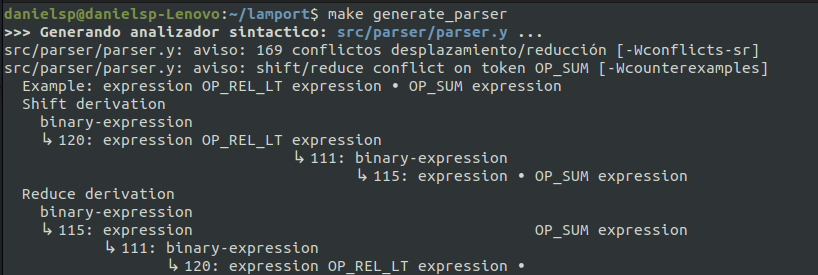
\includegraphics[width=\linewidth]{images/implementacion/parser/parser_conflicts.png}
    \caption{Conflictos de generación de parser por ambigüedad de gramática.}
    \label{fig:parser_conflictos}
\end{figure}

Se producen una inmensa cantidad de conflictos de tipo deslplazamiento/reducción (169 en total). En la captura se observa la indecisión de Bison para decantarse por una regla u otra con el ejemplo:

\begin{verbatim}
    expression OP_REL_LT expression * OP_SUM expression
\end{verbatim}

\noindent
donde se muestran dos caminos posibles para obtener la misma producción.

\vspace{0.5cm}

La solución para este problema en particular pasa por utilizar la precedencia de los operadores que ya se definió en la sección (~\ref{subsec:precOperadoresLamport} ). En Bison se puede indicar utilizando las directivas:

\begin{verbatim}
    %left <TOKEN>
    %right <TOKEN>
\end{verbatim}

\noindent
donde \code{\%left} y \code{\%right} especifican la asociatividad de las operaciones.

\vspace{0.5cm}

\noindent
Aquí se muestra cómo se aplicó la tabla de precedencia en el fichero \code{parser.y}:
\begin{lstlisting}[style=customflex]
%left OP_OR
%left OP_AND
%left OP_REL_EQ OP_REL_NEQ
%left OP_REL_LT OP_REL_LTE OP_REL_GT OP_REL_GTE
%left OP_SUM OP_MINUS
%left OP_MULT OP_DIV OP_MOD
%right OP_NOT

// ....

unary-expression:
    // not term
    OP_NOT term
    // - term
    | OP_MINUS term %prec OP_MINUS
    ;

\end{lstlisting}
\begin{figure}[h]
\caption{Analizador Sintáctico: Especificación de precedencia de operadores en Bison (parser.y)}
\label{fig:bisonPrecOperators}
\end{figure}

Los tokens que se encuentren más abajo en la lista anterior tienen \textbf{mayor prioridad}. Un caso especial es el del operador unario \code{-}, donde debe colocarse explícitamente en la regla donde se utiliza para no confundir a Bison con su homólogo binario.

\vspace{0.5cm}

Ahora el resultado es este, donde ya podemos garantizar que $G$ es una gramática \code{LALR(1)}, que es lo que queríamos demostrar al generar la gramática con Bison:
\begin{figure}[h]
    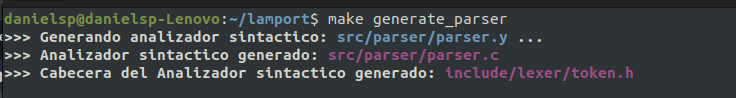
\includegraphics[width=\linewidth]{images/implementacion/parser/parser_success.png}
    \caption{Generación exitosa de la gramática de Lamport.}
    \label{fig:parser_success}
\end{figure}

\subsection{Estrategia de recuperación ante errores sintácticos}
Otro de los problemas a abordar ahora es qué hacer cuando el analizador sintáctico se encuentra con una estructura de tokens que no corresponde con ninguna de las previstas. Aquí hay dos formas posibles de implementar este mecanismo:

\begin{enumerate}
    \item Detectar un error sintáctico y detener inmediatamente el análisis mediante la directiva \code{YYABORT}. Esta acción provoca que, al identificar el primer error en el programa, este sea reconocido y gestionado adecuadamente. Acto seguido, el analizador sintáctico se detendrá, evitando el análisis del resto del fichero.
    
    \item Detectar un error sintáctico e intentar recuperarse, reanudando el análisis a partir de un token específico. En este enfoque, al encontrar un error, se gestiona y, posteriormente, se indica al analizador sintáctico un punto específico dentro de la secuencia de tokens restantes para que continúe con el análisis.
\end{enumerate}

Ambas estrategias son válidas y tienen sus méritos. Sin embargo, es esencial considerar la experiencia del usuario al decidir cuál implementar. La segunda opción, aunque es técnicamente más desafiante debido a la necesidad de identificar los puntos precisos para la recuperación, puede ofrecer una experiencia de usuario más amigable al proporcionar retroalimentación más detallada sobre múltiples errores en lugar de detenerse en el primero.

\vspace{0.5cm}

Independientemente de la estrategia que se implemente, la forma de proceder es la misma, y consiste en definir reglas gramaticales explícitas que se identifiquen como un error sintáctico. A continuación, se muestra un ejemplo para el reconocimiento de errores sintácticos en una declaración de variable:

\begin{lstlisting}[style=customflex]
declaration:
    // ===== CORRECTO: Declaracion completa con asignacion
    S_VAR IDENT DELIM_2P type OP_ASSIGN expression DELIM_PC{
        // ... mas adelante tendra accian semantica ...
    }
    // ===== CORRECTO: Declaracion completa sin asignacion
    | S_VAR IDENT DELIM_2P type DELIM_PC{
        // ... mas adelante tendra accian semantica ...
    }
    // <-> ERROR: se esperaba 'var'
    | IDENT DELIM_2P type DELIM_PC{
        mark_error_syntax_declaration_expected_var($1);
        //YYABORT;
    }
    // <-> ERROR: se esperaba identificador despues de 'var'
    | S_VAR error DELIM_PC{
        mark_error_syntax_declaration_expected_identifier();
        //YYABORT;
    }
    // <-> ERROR: se esperaba ':'
    | S_VAR IDENT error DELIM_PC{
        mark_error_syntax_declaration_expected_delim2p($2);
        //YYABORT;
    };
    // <-> ERROR: se esperaba tipo de dato
    | S_VAR IDENT DELIM_2P DELIM_PC{
        mark_error_syntax_type_expected_type($2);
        //YYABORT;
    }
    // <-> ERROR: se esperaba ';'
    | S_VAR IDENT DELIM_2P type error{
        mark_error_syntax_declaration_expected_delimpc($2);
        //YYABORT;
    }
    // <-> ERROR: se esperaba operador de asignacion
    | S_VAR IDENT DELIM_2P type expression DELIM_PC{
        mark_error_syntax_declaration_expected_opassign($2);
        //YYABORT;
    }
    // <-> ERROR: se esperaba ';'
    | S_VAR IDENT DELIM_2P type OP_ASSIGN expression error{
        mark_error_syntax_declaration_expected_delimpc($2);
        //YYABORT;
    }
    ;

\end{lstlisting}
\begin{figure}[h]
\caption{Analizador Sintáctico: Sección de definición de reglas sintácticas (errores) de Bison (parser.y)}
\label{fig:bisonErrorDeclarations}
\end{figure}

En estas reglas y en todas las definidas para errores, se puede alternar fácilmente entre las estrategias mencionadas comentando o descomentando la directiva \code{YYABORT}. Además, aparece la palabra \code{error}, que es un mecanismo especial en Bison para manejar errores sintácticos. Este mecanismo permite que, en caso de errores, se salte a la parte de la gramática donde se especifica \code{error} para gestionar el fallo y tomar una acción correctiva, ya sea detener el análisis o intentar recuperarse y continuar. Es una herramienta poderosa que proporciona gran flexibilidad en el manejo de errores, permitiendo adaptar la respuesta del analizador a las necesidades específicas del contexto.

\vspace{0.5cm}

Por el momento, se definieron una serie de funciones con mensajes descriptivos en la sección de código C en Bison, que en el producto final desarrollado se movieron a un módulo encargado específicamente de la gestión de errores en el análisis y que se abordará en la sección ~\ref{sec:implementacionError}.

\subsection{Procesamiento de ``Hola Mundo'' utilizando el ``Parser''}\label{subsec:holaMundoParser}

Ahora ya se dispone de un analizador léxico y de un analizador sintáctico, lo que otorga una capacidad de cómputo considerable. Para la interpretación de programas, se utiliza la función \texttt{yyparse()}, que se encarga de iniciar el análisis sintáctico basado en las reglas gramaticales definidas. Antes de invocar a esta función, se asigna al puntero \texttt{yyin} el fichero abierto que contiene el programa, permitiendo que el analizador sintáctico lea el contenido y coordine con el analizador léxico para reconocer los tokens. Finalmente, en la regla de generación del programa completo, se introdujo un mensaje de éxito en su acción semántica. Con estas implementaciones, se procederá a la interpretación del programa ``Hola Mundo'' (~\ref{fig:lamportHolaMundo} ).

\vspace{0.5cm}

Puesto que el programa es sintácticamente correcto, el resultado de la ejecución es el siguiente:

\begin{figure}[h]
\begin{verbatim}
    ``ANÁLISIS SINTÁCTICO REALIZADO CON ÉXITO.''
\end{verbatim}
\caption{Programa ``¡Hola Mundo!'' Lamport: Resultado de análisis sintáctico (simple).}
\label{fig:parserHolaMundo}
\end{figure}

Aunque se ha avanzado significativamente con el analizador sintáctico, aún queda trabajo por hacer. Por ahora, el analizador puede determinar si un programa está bien estructurado o no, y comunicar ese resultado al usuario, pero no es suficiente porque no se realiza un tratamiento específico de cada sección del código Lamport. Por el momento, se han superado los desafíos principales relacionados con la gramática y establecido los módulos de entrada principales. El próximo paso es proporcionar al intérprete de Lamport una estructura que facilite su manipulación computacional: el AST.

\newpage

\section{Árbol de Sintaxis Abstracta (Abstract Syntax Tree,``AST'')}\label{sec:implementacionAST}
Tras completar el análisis sintáctico, surge la necesidad de representar el programa de una manera que facilite su manipulación y análisis en etapas subsecuentes. En este contexto, se introduce el Árbol de Sintaxis Abstracta (AST, por sus siglas en inglés). Un AST proporciona una representación estructurada y jerárquica de la estructura lógica del código fuente, prescindiendo de muchos detalles superficiales presentes en el texto original. En esta sección, se abordará la construcción y características del AST y se profundizará en su relevancia para el entendimiento y procesamiento del programa Lamport.

\subsection{Nodos del AST}
Dentro de la representación de un Árbol de Sintaxis Abstracta (AST), los nodos desempeñan un papel fundamental. Cada nodo refleja una construcción o elemento del lenguaje de programación, y la estructura jerárquica del árbol establece las relaciones entre estos elementos. En esta subsección, se abordarán los diferentes tipos de nodos que componen el AST, sus características y cómo contribuyen a capturar la esencia semántica del programa Lamport.

\vspace{0.5cm}

En la implementación práctica del AST, los nodos se manejan mediante punteros. Esta elección se justifica por diversas razones. Primero, usar punteros permite una gestión dinámica de memoria, lo que facilita la creación, modificación y eliminación de nodos durante el análisis sintáctico. Además, el uso de punteros posibilita la conexión directa entre nodos para formar la estructura de árbol. Esta metodología también optimiza la eficiencia en términos de memoria y acceso, dado que se evita la duplicación de datos y se permite una referencia directa a la información del nodo.

\vspace{0.5cm}
Todos los nodos citados a continuación han sido definidos mediante un \code{struct}, que es una estructura de datos en C que permite agrupar múltiples variables de diferentes tipos bajo un mismo nombre. Estos \code{structs} proporcionan una manera organizada y coherente de representar información compleja. Así, cada nodo del AST puede contener múltiples campos relevantes para su tipo específico, tales como operadores, operandos, identificadores, entre otros. 

\vspace{0.5cm}
De hecho, la estructura subyacente en la mayoría de los nodos (exceptuando el nodo raíz o padre que representa al programa completo) se basa en el concepto de \textbf{lista enlazada}, una estructura de datos muy utilizada en el ámbito de la programación. Esta estructura se emplea con el objetivo de definir secuencias de nodos de manera eficiente, indicando desde cada nodo la posición del siguiente en la lista.

\vspace{0.5cm}
\noindent
Para cada nodo además se implementaron los siguientes grupos de funciones:

\begin{itemize}
    \item \code{struct node * create_node(...)} : Función encargada de reservar memoria e inicializar un nodo en particular teniendo en cuenta los parámetros que se le han pasado a la función.
    \item \code{void free_node(struct node *)} : Función encargada de liberar la memoria reservada para el nodo pasado como parámetro.
    \item \code{void print_node(struct node *, int depth)} : Función encargada de imprimir el contenido del nodo pasado como parámetro en un flujo de salida. El entero \code{depth} especifica la profundidad del nodo en el árbol, para así poder imprimirlo en el lugar donde corresponde.
\end{itemize}



\subsubsection{Nodo de expresión ``expression''}
\noindent
Un nodo de expresión se compone de los siguientes elementos:
\begin{itemize}
    \item \code{expression_t} : tipo de expresión (\code{expression_t} es un enumerado).
    \item \code{char *} : tipo de expresión (en formato \code{string}).
    \item \code{struct expression *} : puntero a siguiente expresión. Útil para encadenar múltiples expresiones.
    \item \code{union} : engloba todas las posibles estructuras para una expresión:

    \begin{itemize}
        \item \code{struct (expression_binary_operation)} : Estructura que contiene todos los campos necesarios para el mantenimiento de una expresión binaria. Contiene:
        \begin{itemize}
            \item \code{expression_binary_t} : tipo de expresión binaria.
            \item \code{char *} : símbolo de operación.
            \item \code{int} : línea de definición de la expresión en el código.
            \item \code{struct expression *} : operando izquierdo de la expresión.
            \item \code{struct expression *} : operando derecho de la expresión.
        \end{itemize}
    \end{itemize}
    \begin{itemize}
        \item \code{struct (expression_unary_expression)} : Estructura que contiene todos los campos necesarios para el mantenimiento de una expresión unaria. Contiene:
        \begin{itemize}
            \item \code{expression_unary_t} : tipo de expresión unaria.
            \item \code{char *} : símbolo de operación.
            \item \code{int} : línea de definición de la expresión en el código.
            \item \code{struct expression *} : operando izquierdo de la expresión (el único que se necesita, pero por convención suele denominarse así).
        \end{itemize}
    \end{itemize}
    \begin{itemize}
        \item \code{struct (expression_identifier)} : Estructura que contiene todos los campos necesarios para el mantenimiento de una expresión de identificador. Contiene:
        \begin{itemize}
            \item \code{char *} nombre de identificador.
            \item \code{struct expression *} : expresión de acceso (útil para accesos a variables de tipo array).
            \item \code{int} : línea de definición de la expresión en el código.
        \end{itemize}
    \end{itemize}
    \begin{itemize}
        \item \code{struct (expression_literal)} : Estructura que contiene todos los campos necesarios para el mantenimiento de una expresión literal. Contiene:
        \begin{itemize}
            \item \code{expression_literal_t} tipo de literal.
            \item \code{union} : contiene los posibles literales: \code{int, float, char, char*, bool}.
        \end{itemize}
    \end{itemize}
    \begin{itemize}
        \item \code{struct (expression_function_inv)} : Estructura que contiene todos los campos necesarios para el mantenimiento de una llamada a función. Contiene:
        \begin{itemize}
            \item \code{char *} nombre de función.
            \item \code{struct expression *} : listado de argumentos de llamada.
            \item \code{int} : línea de definición de la expresión en el código.
        \end{itemize}
    \end{itemize}
    \begin{itemize}
        \item \code{struct expression *} : puntero a expresión que está entre paréntesis \code{()}.
    \end{itemize}
\end{itemize}

\subsubsection{Nodo de tipo de dato ``type''}
\noindent
Un nodo de tipo de dato se compone de los siguientes elementos:
\begin{itemize}
    \item \code{type_t} : tipo de dato (\code{type_t} es un enumerado).
    \item \code{char *} : tipo de dato (en formato \code{string}).
    \item \code{struct type *} : puntero a subtipo de dato, utilizado para arrays.
    \item \code{struct expression *} : línea en la que se define la declaración.
    \item \code{struct type *} : puntero a siguiente tipo, utilizado exclusivamente para definir los tipos de dato de argumentos de una llamada a función o procedimiento.
\end{itemize}

\subsubsection{Nodo de declaración de variable ``declaration''}
\noindent
Un nodo de declaración de variable se compone de los siguientes elementos:
\begin{itemize}
    \item \code{char *} : identificador del nombre de la variable.
    \item \code{struct type *} : puntero al tipo de dato de la variable.
    \item \code{struct expression *} : puntero a la expresión asignada a la variable.
    \item \code{int} : línea en la que se define la declaración.
    \item \code{struct declaration *} : puntero a la siguiente declaración.
\end{itemize}

\subsubsection{Nodo de sentencia ``statement''}
\noindent
Un nodo de sentencia se compone de los siguientes elementos:
\begin{itemize}
    \item \code{statement_t} : tipo de sentencia (\code{statement_t} es un enumerado).
    \item \code{char *} : tipo de sentencia (en formato \code{string}.
    \item \code{struct statement *} : puntero a siguiente sentencia.
    \item \code{union} : engloba todas las posibles estructuras para una sentencia:
    \begin{itemize}
        \item \code{struct (statement_assignment)} : estructura que contiene todos los campos para mantener una sentencia de asignación a variable. Contiene:
        \begin{itemize}
            \item \code{char *}: nombre de variable.
            \item \code{struct expression *}: puntero a expresión de acceso, útil cuando se trata de acceder a una posición específica de un array.
            \item \code{struct expression *}: puntero a expresión de asignación.
        \end{itemize}
    \end{itemize}
    \begin{itemize}
        \item \code{struct (statement_while)} : estructura que contiene todos los campos para mantener una sentencia de bucle while. Contiene:
        \begin{itemize}
            \item \code{struct expression *}: puntero a expresión de condición de bucle.
            \item \code{struct statement *}: puntero a bloque de sentencias de cuerpo de while.
            \item \code{int} : línea de definición de sentencia en el código.
        \end{itemize}
    \end{itemize}
    \begin{itemize}
        \item \code{struct (statement_for)} : estructura que contiene todos los campos para mantener una sentencia de bucle for. Contiene:
        \begin{itemize}
            \item \code{char *}: identificador de índice de bucle.
            \item \code{struct expression *}: puntero a expresión de inicio de bucle.
            \item \code{struct expression *}: puntero a expresión de fin de bucle.
            \item \code{struct statement *}: puntero a bloque de sentencias de cuerpo de for.
            \item \code{int} : línea de definición de sentencia en el código.
        \end{itemize}
    \end{itemize}
    \begin{itemize}
        \item \code{struct (statement_if_else)} : estructura que contiene todos los campos para mantener una sentencia de control if/else. Contiene:
        \begin{itemize}
            \item \code{struct expression *}: puntero a expresión de condición de if.
            \item \code{struct statement *}: puntero a bloque de sentencias de cuerpo de if.
            \item \code{struct statement *}: puntero a bloque de sentencias de cuerpo de else (si dispone).
            \item \code{int} : línea de definición de sentencia en el código.
        \end{itemize}
    \end{itemize}
    \begin{itemize}
        \item \code{struct (statement_procedure_inv)} : estructura que contiene todos los campos para mantener una sentencia de llamada a procedimiento. Contiene:
        \begin{itemize}
            \item \code{char *}: nombre de procedimiento.
            \item \code{struct expression *}: puntero a lista de argumentos de llamada.
            \item \code{int} : línea de definición de sentencia en el código.
        \end{itemize}
    \end{itemize}
    \begin{itemize}
        \item \code{struct (statement_fork)} : estructura que contiene todos los campos para mantener una sentencia de llamada a procedimiento. Contiene:
        \begin{itemize}
            \item \code{char *}: nombre de proceso.
            \item \code{int} : línea de definición de sentencia en el código.
        \end{itemize}
    \end{itemize}
    \begin{itemize}
        \item \code{struct (statement_join)} : estructura que contiene todos los campos para mantener una sentencia de llamada a procedimiento. Contiene:
        \begin{itemize}
            \item \code{char *}: nombre de proceso.
            \item \code{int} : línea de definición de sentencia en el código.
        \end{itemize}
    \end{itemize}
    \begin{itemize}
        \item \code{struct (statement_print)} : estructura que contiene todos los campos para mantener una sentencia de impresión. Contiene:
        \begin{itemize}
            \item \code{struct expression *}: puntero a lista de argumentos de impresión.
        \end{itemize}
    \end{itemize}
    \begin{itemize}
        \item \code{struct (statement_block)} : estructura que encapsula un bloque de sentencias.
    \end{itemize}
\end{itemize}

\subsubsection{Nodo de parámetro de subprograma ``parameter''}
\noindent
Un nodo de parámetro se compone de los siguientes elementos:
\begin{itemize}
    \item \code{char *} : nombre de parámetro.
    \item \code{struct type *} : puntero a tipo de dato.
    \item \code{int *} : línea en la que se define el parámetro.
    \item \code{struct parameter *} : puntero a siguiente parámetro.
\end{itemize}

\subsubsection{Nodo de subprograma ``subprogram''}
\noindent
Un nodo de subprograma se compone de los siguientes elementos:
\begin{itemize}
    \item \code{subprogram_t}: tipo de subprograma (\code{subprogram_t} es un enumerado).
    \item \code{char *}: tipo de subprograma en formato \code{string}.
    \item \code{char *}: nombre de subprograma.
    \item \code{struct parameter *}: puntero a lista de parámetros (si posee).
    \item \code{struct declaration *}: puntero a lista de declaraciones (si posee).
    \item \code{struct statement *}: puntero  lista de sentencias.
    \item \code{struct type *}: puntero a tipo de dato de retorno (sólo funciones).
    \item \code{struct subprogram *}: puntero a siguiente subprograma.
    \item \code{int}: linea de definición de subprograma en el código.
\end{itemize}

\subsubsection{Nodo de proceso ``process''}
\noindent
Un nodo de proceso se compone de los siguientes elementos:
\begin{itemize}
    \item \code{process_t}: tipo de proceso (\code{process_t} es un enumerado).
    \item \code{char *}: tipo de proceso (en formato \code{string}).
    \item \code{char *}: nombre de proceso.
    \item \code{char *}: identificador de índice de proceso (para procesos estáticos vectorizados).
    \item \code{struct expression *}: expresión de inicio de vector de procesos.
    \item \code{struct expression *}: expresión de fin de vector de procesos.
    \item \code{struct declaration *}: lista de declaraciones (si posee).
    \item \code{struct statement *}: lista de sentencias.
    \item \code{int}: línea de definición de proceso en el código.
    \item \code{struct process *}: puntero a siguiente proceso.
\end{itemize}

\subsubsection{Nodo de programa ``program''}
\noindent
Un nodo de programa (el raíz del AST) se compone de los siguientes elementos:
\begin{itemize}
    \item \code{char *}: nombre de programa.
    \item \code{struct subprogram *}: lista de subprogramas (si posee).
    \item \code{struct declaration *}: lista de declaraciones de variables globales (si posee).
    \item \code{struct process *}: lista de procesos.
\end{itemize}

\subsection{Integración del AST en el analizador sintáctico}
Después de definir la estructura y el funcionamiento del AST, hay que usarlo. Manualmente reservar memoria e inicializar nodos no es una estrategia óptima. Es aquí donde las \textbf{acciones semánticas} en las reglas gramaticales de un analizador sintáctico generado por Bison cobran relevancia. Estas acciones semánticas tienen el objetivo de construir el AST a medida que se verifica la sintaxis de los diferentes elementos del lenguaje Lamport.

\vspace{0.5cm}
El primer paso es definir el tipo de dato que devolverán las reglas gramaticales. Para ello se utilizan las directivas:
\begin{verbatim}
    %union
    %type
\end{verbatim}

\vspace{0.5cm}
Con \code{\%union}, Bison identifica los tipos de datos disponibles para las acciones semánticas. Mientras que \code{\%type} permite especificar qué tipo de dato produce cada regla.

\newpage
\begin{figure}[h]
\caption{Analizador Sintáctico: Sección de definición de tipos de reglas en Bison (parser.y)}
\label{fig:bisonASTuniontype}
\end{figure}
\begin{lstlisting}[style=customflex]
// ================================
// ESTRUCTURAS PARA CONSTRUCCION DE AST

%union {
    struct program *prog;
    struct declaration *decl;
    struct subprogram *subprog;
    struct process *proc;
    struct statement *stmt;
    struct expression *expr;
    struct type *type;
    struct parameter *param;
    char *ident;
    char *literal_string;
    char literal_char;
    int literal_int;
    float literal_float;
    int literal_boolean;
};

// ================================
// ESPECIFICACION DE TIPOS DE VALOR SEMANTICO (PARA AST)

// ---- TIPO program
%type <prog> program

// ---- TIPO declaracion
%type <decl> declaration list-declarations

// ---- TIPO subprogram
%type <subprog> list-subprograms subprogram
%type <subprog> subprogram-procedure
%type <subprog> subprogram-function

// ---- TIPO process
%type <proc> list-process process 
%type <proc> process-def process-def-array

// ---- TIPO type
%type <type> type
%type <type> basic-or-array-type
%type <type> basic-type
%type <type> special-type

// ---- TIPO expression
%type <expr> expression 
// ....
%type <expr> expr-identifier
%type <expr> list-arguments argument
%type <expr> list-print

// ---- TIPO parameter
%type <param> list-parameters parameter

// ---- TIPO statement
%type <stmt> statement list-statements
%type <stmt> block-statements-begin-end
// ....
%type <stmt> block-statements-function
%type <stmt> block-statements-process
%type <stmt> assignment-statement 
%type <stmt> while-statement 
// ....
\end{lstlisting}

\vspace{0.5cm}

\noindent
Y ahora, en las reglas podemos definir acciones para construir el AST de forma automática, por ejemplo se muestra la generación del programa y las declaraciones de variables cuando son correctas sintácticamente:

\begin{lstlisting}[style=customflex]
program:
    // ===== CORRECTO: Programa lamport completo
    S_PROGRAM program-name list-declarations list-subprograms list-process{
        // -- Crear AST (solo si no hay errores sintacticos)
        if(!have_syntax_errors())
            AST_program = create_program($2,$3,$4,$5);
    }
    // <-> ERROR: Falta 'program' al comienzo del programa
    | program-name list-declarations list-subprograms list-process{
        mark_error_syntax_program_expected_program($1);
        // -- Abortar inmediatamente el analisis
        //YYABORT;
    }
    // <--> ERROR : Nombre de programa incorrecto
    | S_PROGRAM error list-declarations list-subprograms list-process{
        mark_error_syntax_program_expected_identifier();
        // -- Abortar inmediatamente el analisis
        //YYABORT;
    }
    ;



program-name:
    IDENT{ 
        $$ = $1;
    }
    ;

list-declarations:
    declaration list-declarations{
        if(!have_syntax_errors()){
            $$ = $1;
            $1->next = $2;
        }
        else{
            $$ = 0;
        }
    }
    | /* epsilon */{
        $$ = 0;
    }
    ;

declaration:
    // ===== CORRECTO: Declaracion completa con asignacion
    S_VAR IDENT DELIM_2P type OP_ASSIGN expression DELIM_PC{
        if(!have_syntax_errors()){
            $$ = create_declaration_variable($2, $4, $6, yylineno);
            add_declaration_to_register($$);
        }
        else{
            $$ = 0;
        }
    }
    // ===== CORRECTO: Declaracion completa sin asignacion
    | S_VAR IDENT DELIM_2P type DELIM_PC{
        if(!have_syntax_errors()){
            $$ = create_declaration_variable($2, $4, 0, yylineno);
            add_declaration_to_register($$);
        }
        else{
            $$ = 0;
        }
    }
    // .... (continua el fichero abajo).
\end{lstlisting}
\begin{figure}[h]
\caption{Analizador Sintáctico: Acciones semánticas de reglas gramaticales en Bison (parser.y)}
\label{fig:bisonActionRules}
\end{figure}

Es menester notar que aquí hay un problema a tratar que no es trivial y es parecido a uno que ya se mencionó en la implementación del analizador léxico, y es la correcta gestión de la memoria dinámica, desde la reserva hasta la liberación de los nodos, principalmente cuando el programa es incorrecto en algún punto del código Lamport, pues los nodos que son correctos se crearán y pueden no ser liberados adecuadamente en el caso de encontrarse con un error sintáctico, especialmente si se implementa la estrategia de recuperación de errores y no se decide abortar inmediatamente. 

\vspace{0.5cm}
La solución frente a esto es primero mantener un registro de los nodos que han sido creados para posteriormente liberarlos en cascada sí, y sólo sí, el AST no se ha podido generar por completo. Además, se implementa una guarda que verifica en cada regla correcta si se han producido errores sintácticos en otro punto, y en caso negativo, se genera el nodo correspondiente. En el momento en el que se detecten errores, independientemente de si la sintaxis en líneas posteriores del código es correcta o no, no se generarán más nodos.

\subsection{Procesamiento de ``Hola Mundo'' utilizando el ``Parser'' con AST}
Ahora ya se puede dar forma a nivel estructural y computacional del código Lamport, y es por ello por lo que haciendo el mismo procedimiento que en ~\ref{subsec:holaMundoParser}, se observa ahora que el procesamiento de ``Hola Mundo'' (~\ref{fig:lamportHolaMundo} ) arrojará como resultado el AST que se genere, puesto que el programa es sintácticamente correcto.

\begin{verbatim}
----> PROGRAMA LAMPORT DE NOMBRE: [HolaMundo]
================================================================

----> | DECLARACIONES DE PROGRAMA: [HolaMundo]
|-----> DECLARACION DE VARIABLE: [magico]
|       TIPO DE DATO:
|           TIPO: [integer]
|       VALOR DE INICIALIZACION:
|           <NONE>

================================================================

----> | SUBPROGRAMAS DE PROGRAMA: [HolaMundo]
|-----> NOMBRE DE SUBPROGRAMA: [SaludaUsuario] DE TIPO: [procedure]
|       TIPO DE DATO DE RETORNO:
|   ----> <NONE>
|       PARAMETROS DE SUBPROGRAMA:
|         NOMBRE DE PARAMETRO: [nombre]
|         TIPO DE DATO: [nombre]
|           TIPO: [string]

|       DECLARACIONES DE SUBPROGRAMA:
|-------> <NONE>
|       SENTENCIAS DE SUBPROGRAMA:
|-------> | SENTENCIA DE TIPO: [begin/end block]
|-----------> | SENTENCIA DE TIPO: [print statement]
|             | LISTADO DE EXPRESIONES A IMPRIMIR:
|                > EXPRESION DE TIPO: [literal string]
|                  VALOR DE LITERAL: ["Hola "]
|                > EXPRESION DE TIPO: [identifier]
|                  NOMBRE DE IDENTIFICADOR: [nombre]
|                > EXPRESION DE TIPO: [literal string]
|                  VALOR DE LITERAL: ["!"]



|-----> NOMBRE DE SUBPROGRAMA: [ObtieneNumero] DE TIPO: [function]
|       TIPO DE DATO DE RETORNO:
|         TIPO: [integer]
|       PARAMETROS DE SUBPROGRAMA:
|         NOMBRE DE PARAMETRO: [n]
|         TIPO DE DATO: [n]
|           TIPO: [integer]

|       DECLARACIONES DE SUBPROGRAMA:
|-------> DECLARACION DE VARIABLE: [constant]
|         TIPO DE DATO:
|             TIPO: [integer]
|         VALOR DE INICIALIZACION:
|            > EXPRESION DE TIPO: [binary operation]
|              SIMBOLO DE OPERACION: [-]
|              OPERANDO IZQUIERDO:
|                > EXPRESION DE TIPO: [binary operation]
|                  SIMBOLO DE OPERACION: [*]
|                  OPERANDO IZQUIERDO:
|                    > EXPRESION DE TIPO: [grouped expression]
|                      EXPRESION ENTRE ( )
|                        > EXPRESION DE TIPO: [binary operation]
|                          SIMBOLO DE OPERACION: [+]
|                          OPERANDO IZQUIERDO:
|                            > EXPRESION DE TIPO: [unary operation]
|                              SIMBOLO DE OPERACION: [-]
|                              OPERANDO IZQUIERDO:
|                                > EXPRESION DE TIPO: [literal integer]
|                                  VALOR DE LITERAL: [4]
|                          OPERANDO DERECHO:
|                            > EXPRESION DE TIPO: [literal integer]
|                              VALOR DE LITERAL: [6]
|                  OPERANDO DERECHO:
|                    > EXPRESION DE TIPO: [literal integer]
|                      VALOR DE LITERAL: [10]
|              OPERANDO DERECHO:
|                > EXPRESION DE TIPO: [literal integer]
|                  VALOR DE LITERAL: [2]

|       SENTENCIAS DE SUBPROGRAMA:
|-------> | SENTENCIA DE TIPO: [begin/end block]
|-----------> | SENTENCIA DE TIPO: [return statement]
|             | EXPRESION DE RETORNO:
|                > EXPRESION DE TIPO: [binary operation]
|                  SIMBOLO DE OPERACION: [+]
|                  OPERANDO IZQUIERDO:
|                    > EXPRESION DE TIPO: [identifier]
|                      NOMBRE DE IDENTIFICADOR: [constant]
|                  OPERANDO DERECHO:
|                    > EXPRESION DE TIPO: [identifier]
|                      NOMBRE DE IDENTIFICADOR: [n]



================================================================

----> | PROCESOS DEL PROGRAMA: [HolaMundo]
|-----> | NOMBRE DE PROCESO: [Main] DE TIPO: [individual process]

|-----> | DECLARACIONES DE PROCESO:
|---------> DECLARACION DE VARIABLE: [usuario]
|           TIPO DE DATO:
|               TIPO: [string]
|           VALOR DE INICIALIZACION:
|              > EXPRESION DE TIPO: [literal string]
|                VALOR DE LITERAL: ["Daniel"]

|---------> DECLARACION DE VARIABLE: [numero]
|           TIPO DE DATO:
|               TIPO: [integer]
|           VALOR DE INICIALIZACION:
|              > EXPRESION DE TIPO: [literal integer]
|                VALOR DE LITERAL: [23]


|-----> | SENTENCIAS DE PROCESO:
|---------> | SENTENCIA DE TIPO: [begin/end block]
|-------------> | SENTENCIA DE TIPO: [procedure invocation]
|               | INVOCACION DE PROCEDIMIENTO DE NOMBRE: [SaludaUsuario]
|               | LISTADO DE ARGUMENTOS DE INVOCACION DEL PROCEDIMIENTO:
|                  > EXPRESION DE TIPO: [identifier]
|                    NOMBRE DE IDENTIFICADOR: [usuario]

|-------------> | SENTENCIA DE TIPO: [assignment]
|               | ASIGNACION A VARIABLE: [magico]
|               | EXPRESION ASIGNADA A VARIABLE:
|                  > EXPRESION DE TIPO: [function invocation]
|                    INVOCACION DE FUNCION DE NOMBRE: [ObtieneNumero]
|                    LISTADO DE ARGUMENTOS DE INVOCACION DE FUNCION:
|                      > EXPRESION DE TIPO: [identifier]
|                        NOMBRE DE IDENTIFICADOR: [numero]

|-------------> | SENTENCIA DE TIPO: [print statement]
|               | LISTADO DE EXPRESIONES A IMPRIMIR:
|                  > EXPRESION DE TIPO: [literal string]
|                    VALOR DE LITERAL: ["El numero magico vale: "]
|                  > EXPRESION DE TIPO: [identifier]
|                    NOMBRE DE IDENTIFICADOR: [magico]
\end{verbatim}
\begin{figure}[hbtp]
\caption{Programa ``¡Hola Mundo!'' Lamport: Resultado de análisis sintáctico (AST).}
\label{fig:ASTHolaMundo}
\end{figure}

\newpage

\section{Módulo de análisis semántico: ``Semantic''}\label{sec:implementacionSemantic}
Tras la construcción y análisis del Árbol de Sintaxis Abstracta (AST) mediante el analizador sintáctico, emerge la necesidad de comprender más profundamente el significado de las construcciones presentes en el lenguaje. En esta sección, se introduce el módulo de análisis semántico, que tiene como principal objetivo validar que el programa cumple no solo con las reglas gramaticales del lenguaje Lamport, sino también con las reglas de contexto y las relaciones semánticas que determinan la coherencia y correctitud del código. A través de esta fase, se asegura que el código fuente tiene un sentido lógico y se prepara para las etapas subsiguientes del proceso de interpretación.

\subsection{La tabla de Símbolos}
Dentro del proceso de análisis semántico, es necesario mantener un registro organizado de todas las entidades definidas y utilizadas en el código fuente, desde variables y constantes hasta funciones y procedimientos. Este registro es conocido como la \textbf{tabla de símbolos}. La tabla de símbolos no solo almacena información sobre la declaración de estas entidades, sino también detalles relevantes como su tipo, alcance, y en algunos casos, valores iniciales o información de memoria. Su principal función es facilitar la detección de errores que mencionaremos más adelante.

\subsubsection{Ámbito de variable (scope)}
Uno de los conceptos más fundamentales en la programación y en el análisis semántico es el \textbf{ámbito de una variable}, también conocido como su ``scope''. El ámbito determina en qué partes del código una variable es accesible y dónde puede ser utilizada. Así, dependiendo de dónde se declare una variable, su visibilidad y accesibilidad pueden estar restringidas a un bloque específico de código, a una función o procedimiento, o incluso a todo el programa. Esta característica permite evitar conflictos de nombres y proporciona un grado de encapsulación, esencial para la modularidad y la estructuración de programas complejos.

\vspace{0.5cm}

\noindent
En primer lugar, se definen dos fundamentales ámbitos para una variable:
\begin{itemize}
    \item \textbf{Variable global}: Una variable global es reconocida y accesible por cualquier componente del código Lamport. Se define al principio del programa.
    \item \textbf{Variable local}: Una variable local sólo es reconocida y accesible desde el elemento donde se declaró, que en este caso puede corresponder a un subprograma específico o un proceso.
\end{itemize}

Para realizar un adecuado tratamiento de los ``scopes'', es lógico pensar que la tabla de símbolos no debe contener simplemente símbolos, sino además debe registrarse en qué ambito está definida una determinada variable. Lo más eficiente para hacer esto es considerar una \textbf{tabla Hash} con un tamaño fijo. 

\vspace{0.5cm}
Una tabla hash, también conocida como mapa hash o diccionario, es una estructura de datos que permite asociar pares de clave-valor. Utiliza una función hash para computar un índice en un array de cubetas o ranuras, desde el que se puede localizar el valor deseado. Esta estructura es especialmente útil cuando se desea un acceso rápido a los datos, ya que la función hash tiene como objetivo distribuir las claves de manera uniforme a lo largo de la tabla, permitiendo así una búsqueda, inserción y eliminación de elementos con un tiempo promedio constante. En el contexto de la gestión de ámbitos en la tabla de símbolos, las claves son un número identificador obtenido de aplicar una función hash determinada al nombre del símbolo, siendo el valor que almacena el propio símbolo.

\subsubsection{Implementación de la tabla con una pila de tablas hash}
Para implementar la tabla de forma adecuada teniendo en cuenta los diferentes ``scopes'' posibles en función del número de declaraciones, subprogramas o procesos, la mejor estructura de datos posible es una \textbf{pila de tablas hash}.

\vspace{0.5cm}

Una \textbf{pila de tablas hash} no es más que una colección de tablas hash estructuradas en forma de pila. Cada vez que se entra en un nuevo ámbito (por ejemplo, al ingresar a un subprograma o proceso), se introduce una nueva tabla hash vacía en la cima de la pila. Los símbolos definidos dentro de este ámbito se añaden a esta tabla. Cuando se sale del ámbito, simplemente se retira la tabla hash de la cima de la pila, descartando de esta forma todos los símbolos asociados a ese ámbito en particular.

\vspace{0.5cm}

La ventaja de esta aproximación es que facilita la resolución de referencias a símbolos. Al buscar un símbolo, se empieza por la tabla hash en la cima de la pila (el ámbito actual) y se va descendiendo a través de las tablas de ámbitos exteriores hasta encontrar el símbolo o llegar al fondo de la pila. Esta estructura asegura que siempre se resuelve al símbolo más cercano en términos de ámbito, que es el comportamiento deseado en la mayoría de los lenguajes de programación.

\vspace{0.5cm}

Además, la naturaleza efímera de los ámbitos internos (que se crean y descartan con frecuencia) es manejada de manera natural por la pila. Una vez que se sale de un ámbito, su correspondiente tabla hash se descarta, liberando la memoria y garantizando que los símbolos de ese ámbito no puedan ser referenciados erróneamente en un contexto donde no tienen validez.

{
\centering

\includegraphics[width=200px, height=200px]{images/implementacion/semantic/scope_stack.png}\\
}
\vspace{0.2cm}
Se puede imaginar la tabla de símbolos como una pila de diccionarios donde cada uno contiene símbolos de un único y particular ámbito. Primero se busca en el primer libro que aparece, y si no se encuentra, se va descendiendo poco a poco hasta el final.

\subsection{Resolución de nombres}
La primera fase que debe abordar el analizador semántico es lo que se denomina como \textbf{resolución de nombres}. Esto se refiere a determinar a qué entidad de un programa se refiere un nombre en particular en un contexto dado. Aunque puede parecer trivial, la correcta resolución de nombres es fundamental para garantizar la coherencia y la correcta ejecución del código. 

\vspace{0.5cm}

Para llevar a cabo esta tarea, se deben enfrentar varios desafíos. En primer lugar, es necesario identificar y gestionar los distintos ámbitos o ``scopes'' en los que un nombre puede estar definido. Como se ha visto en secciones anteriores, la estructura de una pila de tablas hash es útil en este aspecto. Cada ámbito tiene su propia tabla hash, y al buscar un nombre, se consulta primero la tabla del ámbito actual, avanzando hacia ámbitos más externos si es necesario.

\vspace{0.5cm}
El esquema general del algoritmo de resolución de nombres es el siguiente, aplicándolo desde el nodo raíz del AST (\code{program}):
\begin{enumerate}
    \item Al inicio del análisis:
    \begin{enumerate}
        \item Insertar el ``scope'' global en la pila.
    \end{enumerate}
    \item Si se trata de un bloque de declaraciones:
    \begin{enumerate}
        \item Comprobar si ya existe un símbolo en la tabla de símbolos para la variable actual a analizar.
        \begin{itemize}
            \item En caso afirmativo, se trata de un \textbf{error de redefinición de variable}.
            \item En otro caso, se crea el símbolo y se inserta en el ``scope''.
        \end{itemize}
        \item Continuar con el resto de variables hasta que no queden.
    \end{enumerate}
    \item Si se trata de un bloque de sentencias/expresiones:
    \begin{itemize}
        \item Aplicar resolución de nombres a cada sentencia o expresión hasta que no queden, buscando en todos los scopes las posibles referencias a símbolos que puedan haber.
        \begin{itemize}
            \item Si no se encuentra una referencia a un símbolo dentro de unas estructuras, se trata de un \textbf{error de uso de símbolo no declarado}, ya sea de variable, subprograma o proceso.
        \end{itemize}
    \end{itemize}
    \item Si se trata de un bloque de subprogramas:
    \begin{enumerate}
        \item Comprobar para el scope global y para el subprograma actual a analizar si ya existe un símbolo en la tabla de símbolos asociado a su identificador.
        \begin{itemize}
            \item En caso afirmativo, se tata de un \textbf{error de redefinición de subprograma}.
            \item En otro caso, se crea el símbolo y se inserta en el ``scope''.
        \end{itemize}
        \item Insertar un nuevo ``scope'' en la pila.
        \item Aplicar resolución de nombres a las declaraciones del subprograma.
        \item Aplicar resolución de nombres a las sentencias del subprograma.
        \item Retirar el ``scope'' actual de la pila.

        \item Continuar con el resto de subprogramas hasta que no queden.
    \end{enumerate}
    \item Si se trata de un bloque de procesos:
    \begin{enumerate}
        \item Comprobar para el scope global y para el proceso actual a analizar si ya existe un símbolo en la tabla de símbolos asociado a su identificador.
        \begin{itemize}
            \item En caso afirmativo, se tata de un \textbf{error de redefinición de proceso}.
            \item En otro caso, se crea el símbolo y se inserta en el ``scope''.
        \end{itemize}
        \item Insertar un nuevo ``scope'' en la pila.
        \item Aplicar resolución de nombres a las declaraciones del proceso.
        \item Aplicar resolución de nombres a las sentencias del proceso.
        \item Retirar el ``scope'' actual de la pila.

        \item Continuar con el resto de procesos hasta que no queden.
    \end{enumerate}
\end{enumerate}

\subsection{Comprobación de tipos}
Esta fase garantiza que las operaciones y asignaciones realizadas en el código fuente son coherentes desde el punto de vista de los tipos de datos involucrados. Así, se evita que, por ejemplo, se intente sumar un número entero con una cadena de texto o que se asigne un valor de tipo real a una variable que espera un valor booleano.

\vspace{0.5cm}

La comprobación de tipos no solo proporciona seguridad en la ejecución al detectar errores potenciales en una etapa temprana del proceso de compilación, sino que también contribuye a la claridad y robustez del código. Aquí es donde entra en juego la descripción semántica que se hizo del lenguaje Lamport en ~\ref{subsec:semanticaLamport}, porque se aplicará directamente en este apartado del analizador semántico.

\vspace{0.5cm}

Con respecto a la comprobación de tipos \textit{per se} no hay ninguna dificultad técnica. La forma de proceder es prácticamente idéntica a la del algoritmo de resolución de nombres, recorriendo el AST comprobando todos los nodos importantes:

\begin{enumerate}
    \item Si se trata de una expresión:
    \begin{itemize}
        \item Comprobar que se verifican todas las restricciones semánticas definidas en ~\ref{subsubsec:restriccionesSemanticas} y que refieren a expresiones.
        \item En caso contrario, se produce un \textbf{error de comprobación de tipos entre operandos de expresión}.
        \item En el caso de una expresión de llamada a función, se debe comprobar que el tipo de los argumentos pasados coincide con el de los parámetros que se definieron para la función, en el mismo orden en el que aparecen éstos.
    \end{itemize}
    \item Si se trata de una declaración de variable y además tiene un valor de inicio:
    \begin{itemize}
        \item Comprobar que el tipo de dato de la variable coincide con la evaluación del tipo de dato que emite la expresión de inicialización.
        \item En caso contrario, se produce un \textbf{error de asignación de tipos}.
    \end{itemize}
    \item Si se trata de un subprograma:
    \begin{itemize}
        \item Comprobar que se verifican todas las restricciones semánticas definidas en ~\ref{subsubsec:restriccionesSemanticas} y que refieren a subprogramas.
        \item En caso contrario, se produce un \textbf{error de comprobación de tipos}.
    \end{itemize}
    \item Si se trata de una sentencia:
    \begin{itemize}
        \item Si se está realizando una sentencia de asignación, mismo tratamiento que en el caso de inicialización de variables.
        \item En el caso de bucles while y estructuras if/else, la expresión de condición debe emitir el tipo \code{boolean}.
        \item En el caso de bucles for, las expresiones de inicio y fin deben emitir el tipo \code{integer}.
        \item En el caso de una llamada a procedimiento, se debe comprobar que el tipo de los argumentos pasados coincide con el de los parámetros que se definieron para el procedimiento, en el mismo orden en el que aparecen éstos.
        \item Todo lo anterior que no se verifique será un \textbf{error de comprobación de tipos ó de asignación}.
    \end{itemize}
\end{enumerate}

\subsection{Procesamiento de ``Hola Mundo'' utilizando el ``Semantic''}
Ahora ya se dispone de todos los analizadores posibles para un lenguaje de programación cualquiera, en particular para el lenguaje Lamport. Adaptando el código del intérprete ahora cuando se supere la fase del analizador sintáctico, se recorrerá el AST generado analizando semánticamente el programa. Primero se aplica resolución de nombres y posteriormente la comprobación de tipos. Si el procesamiento de ``Hola Mundo'' (~\ref{fig:lamportHolaMundo} ) se ha superado, se verá un mensaje de éxito en pantalla. En caso contrario se mostrarán todos los errores semánticos emitidos:

\vspace{0.5cm}

\noindent
Puesto que el programa es semánticamente correcto, el mensaje que se muestra es:
\begin{verbatim}
    ``RESOLUCIÓN DE NOMBRES Y COMPROBACIÓN DE TIPOS 
        REALIZADOS CON ÉXITO.''
\end{verbatim}

\section{Módulo de gestión de errores: ``Error''}\label{sec:implementacionError}
En los módulos de análisis sintáctico (~\ref{sec:implementacionParser} ) y análisis semántico (~\ref{sec:implementacionSemantic} ) se ha comentado la importancia que tiene realizar una gestión adecuada de los errores, y sobretodo, ser transparente en la manera de tratarlos y mostrarlos al usuario del intérprete.

\vspace{0.5cm}
Es por ello que se decidió diseñar un módulo que se encargue específicamente de la gestión de sendos errores, definiendo para ello una estructura común denominada \code{error} que contiene los siguientes campos:

\begin{itemize}
    \item \code{error_type_t}: Especifica el tipo de error (sintáctico o semántico).
    \item \code{int}: Indica la línea en el fichero del código Lamport donde se produjo el error.
    \item \code{msg}: Mensaje de error.
    \item \code{struct error *}: puntero a siguiente error, útil para mostrar múltiples errores.
    \item \code{union}: engloba información adicional sobre los diferentes tipos de error.
    \begin{itemize}
        \item \code{struct (error_syntax)}: contiene información adicional acerca de un error sintáctico:
        \begin{itemize}
            \item \code{error_syntax_t}: tipo de error sintáctico.
            \item \code{char *}: identificador de función, procedimiento, declaración o proceso donde se produjo el error sintáctico.
        \end{itemize}
    \end{itemize}
    \begin{itemize}
        \item \code{struct (error_semantic)}: contiene información adicional acerca de un error semántico:
        \begin{itemize}
            \item \code{error_semantic_t}: tipo de error semántico.
            \item \code{int}: (def\_line) sirve para errores del tipo \textbf{redefinición}, pues se indica en qué parte del fichero de código se definió un determinado símbolo.
            \item \code{int}: (which) también sirve para errores de tipo \textbf{redefinición} cuando se trata de parámetros de subprograma, indicando la posición del parámetro.
            \item \code{char *}: identificador del símbolo que produjo el error semántico.
        \end{itemize}
    \end{itemize}
\end{itemize}

\vspace{0.5cm}
El manejador de errores se integra tanto en el analizador sintáctico como en el semántico. En el primer módulo, las funciones encargadas de marcar los errores se llaman dentro de las reglas sintácticas que son tratadas como errores, mientras que en el segundo módulo simplemente se van realizando llamadas conforme se detecten aplicando los algoritmos descritos anteriormente.

\vspace{0.5cm}
Para finalizar, aquí se muestra el orden en el que aparecen los errores, dependiendo del éxito o no de la superación de las fases de análisis:

\begin{enumerate}
    \item Si no supera el análisis sintáctico, imprimir listado de errores sintácticos producidos.
    \item En caso contrario, si no supera el procedimiento de resolución de nombres, imprimir los errores semánticos producidos.
    \item En caso contrario, si no supera el procedimiento de comprobación de tipos, imprimir los errores semánticos producidos.
\end{enumerate}

\section{Módulo de gestión de Representación Intermedia: ``IR''}\label{sec:implementacionIR}
La transformación y optimización del código fuente en lenguajes de programación suele requerir una etapa intermedia antes de llegar a la fase de generación del código máquina o bytecode, o sencillamente interpretación en el caso particular de este lenguaje. Esta etapa se materializa a través de la Representación Intermedia (IR, por sus siglas en inglés). El módulo ``IR'' se encarga precisamente de gestionar esta representación, que actúa como un puente entre el análisis semántico del código fuente y su traducción final.

\vspace{0.5cm}
Esta representación simplifica y estandariza las operaciones posteriores en el proceso de interpretación, permitiendo optimizaciones y transformaciones sobre una estructura común y coherente. La IR puede adoptar diferentes formas, desde árboles hasta grafos o secuencias de instrucciones, y su diseño adecuado es crucial para el rendimiento y eficacia del intérprete.

\vspace{0.5cm}
A lo largo de esta sección, se describirá la estructura y funcionalidades del módulo ``IR'', así como la importancia y las ventajas de utilizar una Representación Intermedia en el proceso de interpretación.

\subsection{Elección de Representación Intermedia}
Al igual que se realizó un estudio meticuloso para definir el lenguaje Lamport, ahora hay que hacer lo mismo con lenguaje de representación intermedia. Para este proyecto, se optó por una representación intermedia basada en registros, lo cual brinda una organización más clara y directa del flujo de datos y operaciones. Esta elección deriva naturalmente en el uso de \textbf{instrucciones} que detallan cómo se manejan y procesan esos registros. Este enfoque no solo simplifica la representación, sino que además facilita la posterior simulación del funcionamiento de un sistema concurrente en la máquina virtual implementada.

\vspace{0.5cm}
\noindent
Una instrucción consta de los siguientes elementos:

\begin{itemize}
    \item \textbf{Código de instrucción}: Es un identificador que sirve para indicar a la posterior máquina virtual el tipo de instrucción que va a ejecutar.
    \item \textbf{Operando de destino}: Identificador que representa el lugar donde el resultado de la acción que realizará la entidad que ejecute la instrucción se almacenará.
    \item \textbf{Operando 1}: Identificador que representa al dato del primer operando de la instrucción.
    \item \textbf{Operando 2}: Identificador que representa al dato del segundo operando de la instrucción.
\end{itemize}

Los operandos son elementos que determinan las fuentes de datos o valores con los que se realizará la operación indicada por el código de instrucción. Estos pueden ser constantes, registros, direcciones de memoria, entre otros. La cantidad y el tipo de operandos pueden variar según la instrucción, y su correcta interpretación es crucial para el adecuado funcionamiento de la máquina virtual y la ejecución del programa. En esta representación intermedia, hay estos tipos de operandos:

\begin{itemize}
    \item \textbf{Identificación de un registro}: El operando apunta a un registro de la máquina virtual.
    \item \textbf{Identificación de un literal}: El operando apunta a un literal.
    \item \textbf{Identificación de una variable}: El operando apunta a una variable.
    \item \textbf{Identificación de una variable array}: El operando apunta a un elemento en concreto de una variable array.
    \item \textbf{Identificación de una etiqueta}: El operando apunta a la dirección de una etiqueta.
\end{itemize}

Sobre el último tipo de operando mostrado en la enumeración anterior, un aspecto clave en la representación intermedia y su ejecución en la máquina virtual son las \textbf{etiquetas}. En este contexto, una etiqueta no es más que un marcador o referencia que identifica una posición específica dentro del conjunto de instrucciones. Estas etiquetas son imprescindibles para instrucciones de control de flujo, como saltos condicionales o incondicionales, bucles, entre otros.

\vspace{0.5cm}

Por ejemplo, al encontrarse con una instrucción de salto que tiene una etiqueta como operando, la máquina virtual sabe exactamente a qué punto de la lista de instrucciones debe ``saltar'' y continuar con la ejecución desde allí. Las etiquetas, por lo tanto, ofrecen una forma de organizar y controlar el flujo de la ejecución de instrucciones en la representación intermedia, permitiendo la implementación de estructuras lógicas y de control complejas. No obstante, se tratará este aspecto más adelante.

\vspace{0.5cm}
Finalmente, en este lenguaje de representación intermedia hay un total de \textbf{4 tipos de instrucciones diferentes}:

\begin{itemize}
    \item \textbf{1 destino y 2 operandos}: la instrucción a ejecutar necesita de dos operandos y el resultado se almacenará en un destino.
    \item \textbf{1 destino y 1 operando}: la instrucción a ejecutar necesita un operando y el resultado se almacena en un destino.
    \item \textbf{1 operando}: la instrucción a ejecutar necesita un operando, y no hay necesidad de almacenar el resultado de la acción.
    \item \textbf{0 destinos y 0 operandos}: la instrucción sólo dispone de su código de instrucción, suficiente para su ejecución.
\end{itemize}

\subsection{Repertorio de instrucciones de IR}
A continuación se realiza un estudio detallado del repertorio de instrucciones definido para la representación intermedia del lenguaje Lamport.

\renewcommand{\arraystretch}{1.5}
\begin{longtable}{|c|c|c|c|c|}
\caption{Repertorio de instrucciones de Representación Intermedia.} \label{tab:instruccionesIR} \\
\hline
\textbf{CÓDIGO} & \textbf{DETALLES} & \textbf{OP. DESTINO} & \textbf{OP. 1} & \textbf{OP. 2} \\
\hline
\endfirsthead

\multicolumn{5}{c}%
{{\bfseries \tablename\ \thetable{} -- continuación de la página anterior}} \\
\hline
\textbf{CÓDIGO} & \textbf{DETALLES} & \textbf{OP. DESTINO} & \textbf{OP. 1} & \textbf{OP. 2} \\
\hline
\endhead

\hline \multicolumn{5}{|r|}{{Continúa en la siguiente página}} \\
\hline
\endfoot

\hline
\endlastfoot

\code{IR_OP_LOAD} & ~\ref{subsubsec:IR_OP_LOAD}  & SÍ & SÍ & NO \\
\hline
\code{IR_OP_STORE} & ~\ref{subsubsec:IR_OP_STORE} & SÍ & SÍ & NO \\
\hline
\code{IR_OP_ADD} & ~\ref{subsubsec:IR_OP_ADD} & SÍ & SÍ & SÍ \\
\hline
\code{IR_OP_SUB} & ~\ref{subsubsec:IR_OP_SUB} & SÍ & SÍ & SÍ \\
\hline
\code{IR_OP_MULT} & ~\ref{subsubsec:IR_OP_MULT} & SÍ & SÍ & SÍ \\
\hline
\code{IR_OP_DIV} & ~\ref{subsubsec:IR_OP_DIV} & SÍ & SÍ & SÍ \\
\hline
\code{IR_OP_MOD} & ~\ref{subsubsec:IR_OP_MOD} & SÍ & SÍ & SÍ \\
\hline
\code{IR_OP_NEG} & ~\ref{subsubsec:IR_OP_NEG} & SÍ & SÍ & SÍ \\
\hline
\code{IR_OP_AND} & ~\ref{subsubsec:IR_OP_AND} & SÍ & SÍ & SÍ \\
\hline
\code{IR_OP_OR} & ~\ref{subsubsec:IR_OP_OR} & SÍ & SÍ & SÍ \\
\hline
\code{IR_OP_NOT} & ~\ref{subsubsec:IR_OP_NOT} & SÍ & SÍ & SÍ \\
\hline
\code{IR_OP_CMP_LT} & ~\ref{subsubsec:IR_OP_CMP_LT} & SÍ & SÍ & SÍ \\
\hline
\code{IR_OP_CMP_LTE} & ~\ref{subsubsec:IR_OP_CMP_LTE} & SÍ & SÍ & SÍ \\
\hline
\code{IR_OP_CMP_GT} & ~\ref{subsubsec:IR_OP_CMP_GT} & SÍ & SÍ & SÍ \\
\hline
\code{IR_OP_CMP_GTE} & ~\ref{subsubsec:IR_OP_CMP_GTE} & SÍ & SÍ & SÍ \\
\hline
\code{IR_OP_CMP_EQ} & ~\ref{subsubsec:IR_OP_CMP_EQ} & SÍ & SÍ & SÍ \\
\hline
\code{IR_OP_CMP_NEQ} & ~\ref{subsubsec:IR_OP_CMP_NEQ} & SÍ & SÍ & SÍ \\
\hline
\code{IR_OP_JMP} & ~\ref{subsubsec:IR_OP_JMP} & NO & SÍ & NO \\
\hline
\code{IR_OP_JMP_TRUE} & ~\ref{subsubsec:IR_OP_JMP_TRUE} & NO & SÍ & NO \\
\hline
\code{IR_OP_JMP_FALSE} & ~\ref{subsubsec:IR_OP_JMP_FALSE} & NO & SÍ & NO \\
\hline
\code{IR_OP_CALL} & ~\ref{subsubsec:IR_OP_CALL} & NO & SÍ & NO \\
\hline
\code{IR_OP_RET} & ~\ref{subsubsec:IR_OP_RET} & NO & SÍ & NO \\
\hline
\code{IR_OP_PUSH} & ~\ref{subsubsec:IR_OP_PUSH} & NO & SÍ & NO \\
\hline
\code{IR_OP_POP} & ~\ref{subsubsec:IR_OP_POP} & NO & SÍ & NO \\
\hline
\code{IR_OP_PRINT} & ~\ref{subsubsec:IR_OP_PRINT} & NO & SÍ & NO \\
\hline
\code{IR_START_PROGRAM} & ~\ref{subsubsec:IR_START_PROGRAM} & NO & NO & NO \\
\hline
\code{IR_END_PROGRAM} & ~\ref{subsubsec:IR_END_PROGRAM} & NO & NO & NO \\
\hline
\code{IR_START_PROCESS} & ~\ref{subsubsec:IR_START_PROCESS} & NO & NO & NO \\
\hline
\code{IR_END_PROCESS} & ~\ref{subsubsec:IR_END_PROCESS} & NO & NO & NO \\
\hline

\end{longtable}
\renewcommand{\arraystretch}{1.0}


\subsubsection{Instrucción IR\_OP\_LOAD}\label{subsubsec:IR_OP_LOAD}
\noindent
\textbf{Funcionalidad:} Carga un valor de una variable en un registro.

\noindent
\textbf{Argumentos:} La estructura de la instrucción es la siguiente:
\begin{verbatim}
IR_OP_LOAD <registro_destino> <operando1>
\end{verbatim}
\begin{itemize}
    \item <\code{registro_destino}>: registro donde se almacenará el valor de la variable.
    \item <\code{operando1}>: Es una \code{variable}. Su valor se cargará en el registro de destino.
\end{itemize}

\noindent
\textbf{Ejecución de la instrucción:}
\noindent
Se realizan los siguientes pasos para la ejecución de la instrucción:

\begin{enumerate}
    \item El valor de <\code{operando1}> se carga en <\code{registro_destino}>.
\end{enumerate}

\noindent
\textbf{Ejemplo de uso:}
\noindent
Suponiendo que \code{y} es una variable:

\begin{verbatim}
IR_OP_LOAD R1, y
\end{verbatim}

\noindent
\textbf{Comentarios adicionales:}

La representación a nivel de código de esta instrucción realmente contendrá en el operando un entero apuntador a una tabla de variables indexada donde se encuentra el nombre de dicha variable \texttt{y}.

\newpage
\subsubsection{Instrucción IR\_OP\_STORE}\label{subsubsec:IR_OP_STORE}
\noindent
\textbf{Funcionalidad:} Almacena el valor de un registro en una variable.

\noindent
\textbf{Argumentos:} La estructura de la instrucción es la siguiente:

\begin{verbatim}
IR_OP_STORE <registro_fuente> <operando1>
\end{verbatim}
\begin{itemize}
    \item <\code{registro_fuente}>: registro del cual se tomará el valor para almacenarlo en la variable.
    \item <\code{operando1}>: Es una \code{variable}. Se almacenará el valor del registro fuente en esta variable.
\end{itemize}

\noindent
\textbf{Ejecución de la instrucción:}
\noindent
Se realizan los siguientes pasos para la ejecución de la instrucción:

\begin{enumerate}
    \item El valor de <\code{registro_fuente}> se almacena en <\code{operando1}>.
\end{enumerate}

\noindent
\textbf{Ejemplo de uso:}
\noindent
Suponiendo que \code{z} es una variable:

\begin{verbatim}
IR_OP_STORE R2, z
\end{verbatim}

\noindent
\textbf{Comentarios adicionales:}

La representación a nivel de código de esta instrucción realmente contendrá en el operando un entero apuntador a una tabla de variables indexada donde se encuentra el nombre de dicha variable \texttt{z}.

\subsubsection{Instrucción IR\_OP\_ADD}\label{subsubsec:IR_OP_ADD}
\noindent
\textbf{Funcionalidad:} Suma dos operandos y almacena el resultado en un registro.

\noindent
\textbf{Argumentos:} La estructura de la instrucción es la siguiente:
\begin{verbatim}
IR_OP_ADD <registro_destino> <operando1> <operando2>
\end{verbatim}
\begin{itemize}
    \item <\code{registro_destino}>: registro donde se almacenará el resultado de la suma.
    \item <\code{operando1}, \code{operando2}>: Operandos a sumar.
\end{itemize}

\noindent
\textbf{Ejecución de la instrucción:}


\noindent
El valor de <\code{operando1}> se suma al valor de <\code{operando2}>, y el resultado se almacena en <\code{registro_destino}>.


\noindent
\textbf{Ejemplo de uso:}
\begin{verbatim}
IR_OP_ADD R1, R2, R3
\end{verbatim}

\newpage

\subsubsection{Instrucción IR\_OP\_SUB}\label{subsubsec:IR_OP_SUB}
\noindent
\textbf{Funcionalidad:} Resta el segundo operando al primero y almacena el resultado en un registro.

\noindent
\textbf{Argumentos:} La estructura de la instrucción es la siguiente:
\begin{verbatim}
IR_OP_SUB <registro_destino> <operando1> <operando2>
\end{verbatim}
\begin{itemize}
    \item <\code{registro_destino}>: registro donde se almacenará el resultado de la resta.
    \item <\code{operando1}, \code{operando2}>: Operandos involucrados en la resta.
\end{itemize}

\noindent
\textbf{Ejecución de la instrucción:}
\vspace{0.3cm}

\noindent
El valor de <\code{operando2}> se resta del valor de <\code{operando1}>, y el resultado se almacena en <\code{registro_destino}>.
\vspace{0.3cm}

\noindent
\textbf{Ejemplo de uso:}
\begin{verbatim}
IR_OP_SUB R1, R2, R3
\end{verbatim}

\subsubsection{Instrucción IR\_OP\_MULT}\label{subsubsec:IR_OP_MULT}
\noindent
\textbf{Funcionalidad:} Multiplica dos operandos y almacena el resultado en un registro.

\noindent
\textbf{Argumentos:} La estructura de la instrucción es la siguiente:
\begin{verbatim}
IR_OP_MULT <registro_destino> <operando1> <operando2>
\end{verbatim}
\begin{itemize}
    \item <\code{registro_destino}>: registro donde se almacenará el resultado de la multiplicación.
    \item <\code{operando1}, \code{operando2}>: Operandos a multiplicar.
\end{itemize}

\noindent
\textbf{Ejecución de la instrucción:}
\vspace{0.3cm}

\noindent
El valor de <\code{operando1}> se multiplica por el valor de <\code{operando2}>, y el resultado se almacena en <\code{registro_destino}>.
\vspace{0.3cm}

\noindent
\textbf{Ejemplo de uso:}
\begin{verbatim}
IR_OP_MULT R1, R2, R3
\end{verbatim}

\subsubsection{Instrucción IR\_OP\_DIV}\label{subsubsec:IR_OP_DIV}
\noindent
\textbf{Funcionalidad:} Divide el primer operando entre el segundo y almacena el resultado en un registro.

\noindent
\textbf{Argumentos:} La estructura de la instrucción es la siguiente:
\begin{verbatim}
IR_OP_DIV <registro_destino> <operando1> <operando2>
\end{verbatim}
\begin{itemize}
    \item <\code{registro_destino}>: registro donde se almacenará el resultado de la división.
    \item <\code{operando1}, \code{operando2}>: Operandos involucrados en la división.
\end{itemize}

\noindent
\textbf{Ejecución de la instrucción:}
\vspace{0.3cm}

\noindent
El valor de <\code{operando1}> se divide entre el valor de <\code{operando2}>, y el resultado se almacena en <\code{registro_destino}>.
\vspace{0.3cm}

\noindent
\textbf{Ejemplo de uso:}
\begin{verbatim}
IR_OP_DIV R1, R2, R3
\end{verbatim}

\subsubsection{Instrucción IR\_OP\_MOD}\label{subsubsec:IR_OP_MOD}
\noindent
\textbf{Funcionalidad:} Calcula el residuo de la división del primer operando entre el segundo y almacena el resultado en un registro.

\noindent
\textbf{Argumentos:} La estructura de la instrucción es la siguiente:
\begin{verbatim}
IR_OP_MOD <registro_destino> <operando1> <operando2>
\end{verbatim}
\begin{itemize}
    \item <\code{registro_destino}>: registro donde se almacenará el resultado del cálculo del residuo.
    \item <\code{operando1}, \code{operando2}>: Operandos involucrados en el cálculo del residuo.
\end{itemize}

\noindent
\textbf{Ejecución de la instrucción:}
\vspace{0.3cm}

\noindent
El residuo de la división del valor de <\code{operando1}> entre el valor de <\code{operando2}> se calcula, y el resultado se almacena en <\code{registro_destino}>.
\vspace{0.3cm}

\noindent
\textbf{Ejemplo de uso:}
\begin{verbatim}
IR_OP_MOD R1, R2, R3
\end{verbatim}

\subsubsection{Instrucción IR\_OP\_NEG}\label{subsubsec:IR_OP_NEG}
\noindent
\textbf{Funcionalidad:} Realiza la negación aritmética del operando y almacena el resultado en un registro.

\noindent
\textbf{Argumentos:} La estructura de la instrucción es la siguiente:
\begin{verbatim}
IR_OP_NEG <registro_destino> <operando1>
\end{verbatim}
\begin{itemize}
    \item <\code{registro_destino}>: registro donde se almacenará el resultado de la negación.
    \item <\code{operando1}>: operando a negar.
\end{itemize}

\noindent
\textbf{Ejecución de la instrucción:}
\vspace{0.3cm}

\noindent
Se niega el valor de <\code{operando1}> y el resultado se almacena en \\
<\code{registro_destino}>.
\vspace{0.3cm}

\noindent
\textbf{Ejemplo de uso:}
\begin{verbatim}
IR_OP_NEG R0, R1
\end{verbatim}

\subsubsection{Instrucción IR\_OP\_AND}\label{subsubsec:IR_OP_AND}
\noindent
\textbf{Funcionalidad:} Realiza la conjunción lógica entre dos operandos y almacena el resultado en un registro.

\noindent
\textbf{Argumentos:} La estructura de la instrucción es la siguiente:
\begin{verbatim}
IR_OP_AND <registro_destino> <operando1> <operando2>
\end{verbatim}
\begin{itemize}
    \item <\code{registro_destino}>: registro donde se almacenará el resultado de la conjunción lógica.
    \item <\code{operando1}, \code{operando2}>: operandos de la conjunción lógica.
\end{itemize}

\noindent
\textbf{Ejecución de la instrucción:}
\vspace{0.3cm}

\noindent
Se realiza AND lógico entre los valores de <\code{operando1}> y <\code{operando2}> y el resultado se almacena en <\code{registro_destino}>.
\vspace{0.3cm}

\noindent
\textbf{Ejemplo de uso:}
\begin{verbatim}
IR_OP_AND R0, R1, $true
\end{verbatim}

\subsubsection{Instrucción IR\_OP\_OR}\label{subsubsec:IR_OP_OR}
\noindent
\textbf{Funcionalidad:} Realiza la disyunción lógica entre dos operandos y almacena el resultado en un registro.

\noindent
\textbf{Argumentos:} La estructura de la instrucción es la siguiente:
\begin{verbatim}
IR_OP_OR <registro_destino> <operando1> <operando2>
\end{verbatim}
\begin{itemize}
    \item <\code{registro_destino}>: registro donde se almacenará el resultado de la disyunción lógica.
    \item <\code{operando1}, \code{operando2}>: operandos de la disyunción lógica.
\end{itemize}

\noindent
\textbf{Ejecución de la instrucción:}
\vspace{0.3cm}

\noindent
Se realiza OR lógico entre los valores de <\code{operando1}> y <\code{operando2}> y el resultado se almacena en <\code{registro_destino}>.
\vspace{0.3cm}

\noindent
\textbf{Ejemplo de uso:}
\begin{verbatim}
IR_OP_OR R0, R1, R2
\end{verbatim}

\subsubsection{Instrucción IR\_OP\_NOT}\label{subsubsec:IR_OP_NOT}
\noindent
\textbf{Funcionalidad:} Realiza la negación lógica de un operando y almacena el resultado en un registro.

\noindent
\textbf{Argumentos:} La estructura de la instrucción es la siguiente:
\begin{verbatim}
IR_OP_NOT <registro_destino> <operando1>
\end{verbatim}
\begin{itemize}
    \item <\code{registro_destino}>: registro donde se almacenará el resultado de la operación lógica.
    \item <\code{operando1}>: operando de negación lógica. Puede ser: registro, literal.
\end{itemize}

\noindent
\textbf{Ejecución de la instrucción:}
\vspace{0.3cm}

\noindent
Se realiza NOT lógico de <\code{operando1}> y el resultado se almacena en <\code{registro_destino}>.
\vspace{0.3cm}

\noindent
\textbf{Ejemplo de uso:}
\begin{verbatim}
IR_OP_NOT R0, R1
\end{verbatim}


\subsubsection{Instrucción IR\_OP\_CMP\_LT}\label{subsubsec:IR_OP_CMP_LT}
\noindent
\textbf{Funcionalidad:} Compara si un operando es menor que otro y almacena el resultado de la comparación en un registro. El resultado será TRUE o FALSE.

\noindent
\textbf{Argumentos:} La estructura de la instrucción es la siguiente:
\begin{verbatim}
IR_OP_CMP_LT <registro_destino> <operando1> <operando2>
\end{verbatim}
\begin{itemize}
    \item <\code{registro_destino}>: registro donde se almacenará el resultado de la operación de comparación.
    \item <\code{operando1}> y <\code{operando2}>: operandos de comparación. Pueden ser: registro, literal.
\end{itemize}

\noindent
\textbf{Ejecución de la instrucción:}
\vspace{0.3cm}

\noindent
Se compara si <\code{operando1}> es menor que <\code{operando2}> y el resultado se almacena en <\code{registro_destino}>.
\vspace{0.3cm}

\noindent
\textbf{Ejemplo de uso:}
\begin{verbatim}
IR_OP_CMP_LT R0, R1, $5
\end{verbatim}

\newpage
\subsubsection{Instrucción IR\_OP\_CMP\_LTE}\label{subsubsec:IR_OP_CMP_LTE}
\noindent
\textbf{Funcionalidad:} Compara si un operando es menor o igual que otro y almacena el resultado de la comparación en un registro. El resultado será TRUE o FALSE.

\noindent
\textbf{Argumentos:} La estructura de la instrucción es la siguiente:
\begin{verbatim}
IR_OP_CMP_LTE <registro_destino> <operando1> <operando2>
\end{verbatim}
\begin{itemize}
    \item <\code{registro_destino}>: registro donde se almacenará el resultado de la operación de comparación.
    \item <\code{operando1}> y <\code{operando2}>: operandos de comparación. Pueden ser: registro, literal.
\end{itemize}

\noindent
\textbf{Ejecución de la instrucción:}
\vspace{0.3cm}

\noindent
Se compara si <\code{operando1}> es menor o igual que <\code{operando2}> y el resultado se almacena en <\code{registro_destino}>.
\vspace{0.3cm}

\noindent
\textbf{Ejemplo de uso:}
\begin{verbatim}
IR_OP_CMP_LTE R0, R1, $5
\end{verbatim}

\subsubsection{Instrucción IR\_OP\_CMP\_GT}\label{subsubsec:IR_OP_CMP_GT}
\noindent
\textbf{Funcionalidad:} Compara si un operando es mayor que otro y almacena el resultado de la comparación en un registro. El resultado será TRUE o FALSE.

\noindent
\textbf{Argumentos:} La estructura de la instrucción es la siguiente:
\begin{verbatim}
IR_OP_CMP_GT <registro_destino> <operando1> <operando2>
\end{verbatim}
\begin{itemize}
    \item <\code{registro_destino}>: registro donde se almacenará el resultado de la operación de comparación.
    \item <\code{operando1}> y <\code{operando2}>: operandos de comparación. Pueden ser: registro, literal.
\end{itemize}

\noindent
\textbf{Ejecución de la instrucción:}
\vspace{0.3cm}

\noindent
Se compara si <\code{operando1}> es mayor que <\code{operando2}> y el resultado se almacena en <\code{registro_destino}>.
\vspace{0.3cm}

\noindent
\textbf{Ejemplo de uso:}
\begin{verbatim}
IR_OP_CMP_GT R0, R1, $5
\end{verbatim}

\subsubsection{Instrucción IR\_OP\_CMP\_GTE}\label{subsubsec:IR_OP_CMP_GTE}
\noindent
\textbf{Funcionalidad:} Compara si un operando es mayor o igual que otro y almacena el resultado de la comparación en un registro. El resultado será TRUE o FALSE.

\noindent
\textbf{Argumentos:} La estructura de la instrucción es la siguiente:
\begin{verbatim}
IR_OP_CMP_GTE <registro_destino> <operando1> <operando2>
\end{verbatim}
\begin{itemize}
    \item <\code{registro_destino}>: registro donde se almacenará el resultado de la operación de comparación.
    \item <\code{operando1}> y <\code{operando2}>: operandos de comparación. Pueden ser: registro, literal.
\end{itemize}

\noindent
\textbf{Ejecución de la instrucción:}
\vspace{0.3cm}

\noindent
Se compara si <\code{operando1}> es mayor o igual que <\code{operando2}> y el resultado se almacena en <\code{registro_destino}>.
\vspace{0.3cm}

\noindent
\textbf{Ejemplo de uso:}
\begin{verbatim}
IR_OP_CMP_GTE R0, R1, $5
\end{verbatim}


\subsubsection{Instrucción IR\_OP\_CMP\_EQ}\label{subsubsec:IR_OP_CMP_EQ}
\noindent
\textbf{Funcionalidad:} Compara si un operando es igual que otro y almacena el resultado de la comparación en un registro. El resultado será TRUE o FALSE.

\noindent
\textbf{Argumentos:} La estructura de la instrucción es la siguiente:
\begin{verbatim}
IR_OP_CMP_EQ <registro_destino> <operando1> <operando2>
\end{verbatim}
\begin{itemize}
    \item <\code{registro_destino}>: registro donde se almacenará el resultado de la operación de comparación.
    \item <\code{operando1}> y <\code{operando2}>: operandos de comparación. Pueden ser: registro, literal.
\end{itemize}

\noindent
\textbf{Ejecución de la instrucción:}
\vspace{0.3cm}

\noindent
Se compara si <\code{operando1}> es igual que <\code{operando2}> y el resultado se almacena en <\code{registro_destino}>.
\vspace{0.3cm}

\noindent
\textbf{Ejemplo de uso:}
\begin{verbatim}
IR_OP_CMP_EQ R0, R1, $5
\end{verbatim}

\subsubsection{Instrucción IR\_OP\_CMP\_NEQ}\label{subsubsec:IR_OP_CMP_NEQ}
\noindent
\textbf{Funcionalidad:} Compara si un operando es distinto que otro y almacena el resultado de la comparación en un registro. El resultado será TRUE o FALSE.

\noindent
\textbf{Argumentos:} La estructura de la instrucción es la siguiente:
\begin{verbatim}
IR_OP_CMP_NEQ <registro_destino> <operando1> <operando2>
\end{verbatim}
\begin{itemize}
    \item <\code{registro_destino}>: registro donde se almacenará el resultado de la operación de comparación.
    \item <\code{operando1}> y <\code{operando2}>: operandos de comparación. Pueden ser: registro, literal.
\end{itemize}

\noindent
\textbf{Ejecución de la instrucción:}
\vspace{0.3cm}

\noindent
Se compara si <\code{operando1}> es distinto que <\code{operando2}> y el resultado se almacena en <\code{registro_destino}>.
\vspace{0.3cm}

\noindent
\textbf{Ejemplo de uso:}
\begin{verbatim}
IR_OP_CMP_NEQ R0, R1, $5
\end{verbatim}

\subsubsection{Instrucción IR\_OP\_JMP}\label{subsubsec:IR_OP_JMP}
\noindent
\textbf{Funcionalidad:} Realiza un salto incondicional a la etiqueta especificada.

\noindent
\textbf{Argumentos:}
\begin{verbatim}
IR_OP_JMP <operando1>
\end{verbatim}
\begin{itemize}
    \item <\code{operando1}>: operando de salto. Es una \textit{etiqueta} que indica la entrada de un bloque de instrucciones.
\end{itemize}

\noindent
\textbf{Ejecución de la instrucción:}
\vspace{0.3cm}

\noindent
La ejecución se desplaza inmediatamente a la instrucción marcada por <\code{operando1}>.
\vspace{0.3cm}

\noindent
\textbf{Ejemplo de uso:}
\begin{verbatim}
IR_OP_JMP etq1
\end{verbatim}

\subsubsection{Instrucción IR\_OP\_JMP\_TRUE}\label{subsubsec:IR_OP_JMP_TRUE}
\noindent
\textbf{Funcionalidad:} Realiza un salto condicional a la etiqueta especificada si el valor de un registro es verdadero.

\noindent
\textbf{Argumentos:}
\begin{verbatim}
IR_OP_JMP_TRUE <operando1> <operando2>
\end{verbatim}
\begin{itemize}
    \item <\code{operando1}>: operando que contiene valor a evaluar (bool). Es un \textit{registro}.
    \item <\code{operando2}>: operando de salto. Es una \textit{etiqueta} que indica la entrada de un bloque de instrucciones.
\end{itemize}

\noindent
\textbf{Ejecución de la instrucción:}
\vspace{0.3cm}

\noindent
La ejecución se desplaza a la instrucción marcada por la etiqueta en <\code{operando2}> sólo si la evaluación del valor del registro en <\code{operando1}> es verdadero.
\vspace{0.3cm}

\noindent
\textbf{Ejemplo de uso:}
\begin{verbatim}
IR_OP_JMP_TRUE R0, etq2
\end{verbatim}

\subsubsection{Instrucción IR\_OP\_JMP\_FALSE}\label{subsubsec:IR_OP_JMP_FALSE}
\noindent
\textbf{Funcionalidad:} Realiza un salto condicional a la etiqueta especificada si el valor de un registro es falso.

\noindent
\textbf{Argumentos:}
\begin{verbatim}
IR_OP_JMP_FALSE <operando1> <operando2>
\end{verbatim}
\begin{itemize}
    \item <\code{operando1}>: operando que contiene valor a evaluar (bool). Es un \textit{registro}.
    \item <\code{operando2}>: operando de salto. Es una \textit{etiqueta} que indica la entrada de un bloque de instrucciones.
\end{itemize}

\noindent
\textbf{Ejecución de la instrucción:}
\vspace{0.3cm}

\noindent
La ejecución se desplaza a la instrucción marcada por la etiqueta en <\code{operando2}> sólo si la evaluación del valor del registro en <\code{operando1}> es falso.
\vspace{0.3cm}

\noindent
\textbf{Ejemplo de uso:}
\begin{verbatim}
IR_OP_JMP_FALSE R0, etq2
\end{verbatim}

\subsubsection{Instrucción IR\_OP\_CALL}\label{subsubsec:IR_OP_CALL}
\noindent
\textbf{Funcionalidad:} Realiza una llamada a un subprograma.

\noindent
\textbf{Argumentos:}
\begin{verbatim}
IR_OP_CALL <operando1>
\end{verbatim}
\begin{itemize}
    \item <\code{operando1}>: operando que indica el inicio de subprograma. Es una \textit{etiqueta}.
\end{itemize}

\noindent
\textbf{Ejecución de la instrucción:}
\vspace{0.3cm}

\noindent
Se guardan el contexto actual (dirección de retorno, registros,...) y la ejecución se desplaza al inicio del subprograma, indicado por el <\code{operando1}>.
\vspace{0.3cm}

\noindent
\textbf{Ejemplo de uso:}
\begin{verbatim}
IR_OP_CALL subprog_etq
\end{verbatim}

\subsubsection{Instrucción IR\_OP\_RET}\label{subsubsec:IR_OP_RET}
\noindent
\textbf{Funcionalidad:} Realiza un retorno de un subprograma.

\noindent
\textbf{Argumentos:}
\begin{verbatim}
IR_OP_RET
\end{verbatim}

\noindent
\textbf{Ejecución de la instrucción:}
\vspace{0.3cm}

\noindent
Se restaura el contexto guardado con anterioridad producido por una instrucción \texttt{IR\_OP\_CALL} y se desplaza la ejecución al punto justo después de la instrucción \texttt{IR\_OP\_CALL} realizada.
\vspace{0.3cm}

\noindent
\textbf{Ejemplo de uso:}
\begin{verbatim}
IR_OP_RET
\end{verbatim}


\subsubsection{Instrucción IR\_OP\_PUSH}\label{subsubsec:IR_OP_PUSH}
\noindent
\textbf{Funcionalidad:} Empuja un valor desde un registro específico a la pila de ejecución.

\noindent
\textbf{Argumentos:}
\begin{verbatim}
IR_OP_PUSH <operando1>
\end{verbatim}
\begin{itemize}
    \item <\code{operando1}>: operando que indica el valor. Es un \textit{registro}.
\end{itemize}

\noindent
\textbf{Ejecución de la instrucción:}
\vspace{0.3cm}

\noindent
Se leen el valor actual del registro especificado y se empuja este valor al tope de la pila de ejecución.
\vspace{0.3cm}

\noindent
\textbf{Ejemplo de uso:}
\begin{verbatim}
IR_OP_PUSH R1
\end{verbatim}

\subsubsection{Instrucción IR\_OP\_POP}\label{subsubsec:IR_OP_POP}
\noindent
\textbf{Funcionalidad:} Desapila el valor del tope de la pila de ejecución y lo almacena en un registro específico.

\noindent
\textbf{Argumentos:}
\begin{verbatim}
IR_OP_POP <operando1>
\end{verbatim}
\begin{itemize}
    \item <\code{operando1}>: operando que indica el lugar de almacenamiento. Es un \textit{registro}.
\end{itemize}

\noindent
\textbf{Ejecución de la instrucción:}
\vspace{0.3cm}

\noindent
Se desapila el valor del tope de la pila de ejecución y se almacena este valor en el registro especificado.
\vspace{0.3cm}

\noindent
\textbf{Ejemplo de uso:}
\begin{verbatim}
IR_OP_POP R1
\end{verbatim}

\subsubsection{Instrucción IR\_OP\_PRINT}\label{subsubsec:IR_OP_PRINT}
\noindent
\textbf{Funcionalidad:} Imprime el valor de un registro o literal en la salida estándar.

\noindent
\textbf{Argumentos:}
\begin{verbatim}
IR_OP_PRINT <operando1>
\end{verbatim}
\begin{itemize}
    \item <\code{operando1}>: Operando de impresión con el valor que se desea imprimir. Es un \textit{registro} o \textit{literal}.
\end{itemize}

\noindent
\textbf{Ejecución de la instrucción:}
\vspace{0.3cm}

\noindent
Se imprime el valor de <\code{operando1}>.
\vspace{0.3cm}

\noindent
\textbf{Ejemplo de uso:}
\begin{verbatim}
IR_OP_PRINT R0
IR_OP_PRINT $"hola"
\end{verbatim}


\subsubsection{Instrucción IR\_START\_PROGRAM}\label{subsubsec:IR_START_PROGRAM}
\noindent
\textbf{Funcionalidad:} Indica el inicio de un programa Lamport.

\noindent
\textbf{Argumentos:}
\begin{verbatim}
IR_START_PROGRAM
\end{verbatim}

\noindent
\textbf{Ejecución de la instrucción:}
\vspace{0.3cm}

\noindent
//TODO
\vspace{0.3cm}

\noindent
\textbf{Ejemplo de uso:}
\begin{verbatim}
IR_START_PROGRAM
\end{verbatim}

\subsubsection{Instrucción IR\_END\_PROGRAM}\label{subsubsec:IR_END_PROGRAM}
\noindent
\textbf{Funcionalidad:} Indica el fin de un programa Lamport.

\noindent
\textbf{Argumentos:}
\begin{verbatim}
IR_END_PROGRAM
\end{verbatim}

\noindent
\textbf{Ejecución de la instrucción:}
\vspace{0.3cm}

\noindent
//TODO
\vspace{0.3cm}

\noindent
\textbf{Ejemplo de uso:}
\begin{verbatim}
IR_END_PROGRAM
\end{verbatim}

\subsubsection{Instrucción IR\_START\_PROCESS}\label{subsubsec:IR_START_PROCESS}
\noindent
\textbf{Funcionalidad:} Indica el inicio de un proceso Lamport.

\noindent
\textbf{Argumentos:}
\begin{verbatim}
IR_START_PROCESS
\end{verbatim}

\noindent
\textbf{Ejecución de la instrucción:}
\vspace{0.3cm}

\noindent
//TODO
\vspace{0.3cm}

\noindent
\textbf{Ejemplo de uso:}
\begin{verbatim}
IR_START_PROCESS
\end{verbatim}

\subsubsection{Instrucción IR\_END\_PROCESS}\label{subsubsec:IR_END_PROCESS}
\noindent
\textbf{Funcionalidad:} Indica el fin de un proceso Lamport.

\noindent
\textbf{Argumentos:}
\begin{verbatim}
IR_END_PROCESS
\end{verbatim}

\noindent
\textbf{Ejecución de la instrucción:}
\vspace{0.3cm}

\noindent
//TODO
\vspace{0.3cm}

\noindent
\textbf{Ejemplo de uso:}
\begin{verbatim}
IR_END_PROCESS
\end{verbatim}

\subsection{Organización de elementos del código en tablas}
Dentro del ámbito de la implementación de sistemas, y más específicamente en el contexto de compiladores e intérpretes, la organización de elementos del código en estructuras tabulares es una práctica común. Estas estructuras, denominadas a menudo como tablas de descriptores, juegan un papel crucial en la traducción y optimización del código.

\subsubsection{Tabla de literales}
Se almacenan en una tabla que relaciona cada literal con un índice único. Durante el proceso de interpretación, al encontrar un literal en el código fuente, este se referencia mediante su índice en dicha tabla.

\subsubsection{Tabla de variables}
Las variables declaradas en el código fuente se organizan en una estructura tabular similar. Esta tabla, además de contener el nombre de la variable alberga información adicional como su tipo, su alcance y valor de inicio. A cada entrada en la tabla de variables se le asigna un índice único, que se utiliza para referenciar la variable en las etapas subsiguientes del proceso de interpretación.

\subsubsection{Tabla de etiquetas}
Al detectar una etiqueta en el código, esta se asocia a un índice en la tabla de etiquetas, lo que permite que posteriormente se haga referencia a dicha etiqueta a través de su índice y no por su nombre completo.

\subsubsection{Analogía con la Memoria Virtual}
La técnica de indexación y referencia de elementos mediante tablas guarda similitud con el principio de memoria virtual en sistemas operativos. En este último, las direcciones usadas por un programa (direcciones virtuales) no se traducen directamente en direcciones físicas de la memoria principal. En cambio, se emplean tablas de páginas que facilitan la traducción de direcciones virtuales a físicas. De forma análoga, en las tablas de literales, etiquetas y variables, los índices actúan como referencias intermedias que se resuelven posteriormente. Este será el mecanismo empleado para la organización de la memoria de la máquina virtual, de la que se hablará en la siguiente sección.

\subsection{Optimizaciones de código: Constant Folding}
En el ámbito de la compilación y generación de código, la optimización es una fase crucial, especialmente para reducir el número de instrucciones necesarias para la ejecución de un programa. En este proyecto se ha considerado implementar el algoritmo de \textbf{Constant Folding} para reducir la dimensión de las expresiones.

\vspace{0.5cm}
``Constant Folding'' se refiere al proceso de evaluar expresiones constantes en tiempo de compilación. Es decir, en lugar de esperar que estas expresiones se evalúen en tiempo de ejecución, se resuelven anticipadamente, lo que conlleva a un código más eficiente y a una ejecución más rápida.

\vspace{0.5cm}
Por ejemplo, considere la expresión en el código fuente: \code{int x = 5 * 10;}. Un compilador que aplica ``Constant Folding'' transformará esta expresión en \code{int x = 50;} durante la fase de optimización. Las ventajas que tiene hacer esto son las siguientes:

\begin{itemize}
    \item \textbf{Reducción de la carga computacional:} Al evaluar expresiones en tiempo de compilación, se ahorra el tiempo y esfuerzo necesario para calcularlas en tiempo de ejecución.
    \item \textbf{Reducción del tamaño del código:} Al resolver las expresiones constantes, se pueden eliminar operaciones redundantes y, por lo tanto, se puede generar un código más conciso.
\end{itemize}

\vspace{0.5cm}
\noindent
Aquí se muestra un pseudocódigo de cómo es el algoritmo de ``Constant Folding'' \cite[Capítulo 8]{thain2020introduction}:
\begin{verbatim}
ConstantFold( Node n ):
    If n is a leaf:
        return;
    Else:
        n.left = ConstantFold(n.left);
        n.right = ConstantFold(n.right);
    
    If n.left and n.right are constants:
        n.value = n.operator(n.left,n.right);
        n.kind = constant;
        delete n.left and n.right;
\end{verbatim}

En el programa ``Hola Mundo'' (~\ref{fig:lamportHolaMundo} ), la variable \code{constant} declarada para la función \code{ObtieneNumero} (línea 10), está inicializada mediante una expresión aritmética: \begin{verbatim}
    (-4 + 6) * 10 - 2;
\end{verbatim}

o lo que es lo mismo, el valor \code{18}. El trozo de AST correspondiente a esta parte en cuestión es el siguiente:

\begin{verbatim}
|-------> DECLARACION DE VARIABLE: [constant]
|         TIPO DE DATO:
|             TIPO: [integer]
|         VALOR DE INICIALIZACION:
|            > EXPRESION DE TIPO: [binary operation]
|              SIMBOLO DE OPERACION: [-]
|              OPERANDO IZQUIERDO:
|                > EXPRESION DE TIPO: [binary operation]
|                  SIMBOLO DE OPERACION: [*]
|                  OPERANDO IZQUIERDO:
|                    > EXPRESION DE TIPO: [grouped expression]
|                      EXPRESION ENTRE ( )
|                        > EXPRESION DE TIPO: [binary operation]
|                          SIMBOLO DE OPERACION: [+]
|                          OPERANDO IZQUIERDO:
|                            > EXPRESION DE TIPO: [unary operation]
|                              SIMBOLO DE OPERACION: [-]
|                              OPERANDO IZQUIERDO:
|                                > EXPRESION DE TIPO: [literal integer]
|                                  VALOR DE LITERAL: [4]
|                          OPERANDO DERECHO:
|                            > EXPRESION DE TIPO: [literal integer]
|                              VALOR DE LITERAL: [6]
|                  OPERANDO DERECHO:
|                    > EXPRESION DE TIPO: [literal integer]
|                      VALOR DE LITERAL: [10]
|              OPERANDO DERECHO:
|                > EXPRESION DE TIPO: [literal integer]
|                  VALOR DE LITERAL: [2]
\end{verbatim}

Visualmente ya es demasiado grande, por lo que evidentemente si se procesa esta declaración la cantidad de instrucciones a definir sólo para esta operación de asignación será absurdamente elevada. No obstante, el motivo por lo que se muestra así al usuario es para que aprenda el funcionamiento de un intérprete en cualquier fase del mismo, aunque internamente opere con optimizaciones.

\vspace{0.5cm}

Sin embargo, si se imprime el AST justo después de aplicar el algoritmo de ``Constant Folding'' el resultado es el siguiente:

\begin{verbatim}
|-------> DECLARACION DE VARIABLE: [constant]
|         TIPO DE DATO:
|             TIPO: [integer]
|         VALOR DE INICIALIZACION:
|            > EXPRESION DE TIPO: [literal integer]
|              VALOR DE LITERAL: [18]

\end{verbatim}

puesto que ha evaluado la expresión justo antes de generar instrucciones y se ha reducido al máximo el tamaño de la expresión, donde ahora sólo será necesaria una instrucción de carga.

\subsection{Asignación de registros}\label{subsec:asignacionRegIR}
La asignación de registros es una técnica fundamental en la fase de generación de código de un compilador. Su objetivo principal es mapear variables y resultados intermedios a registros de la máquina objetivo con el propósito de maximizar la eficiencia en la ejecución del código.

\vspace{0.5cm}
Puesto que la representación intermedia elegida es \textit{basada en registros}, es evidente que es necesario en este punto definir una estrategia para la asignación de los mismos, y hay dos formas de implementarlo:

\begin{enumerate}
    \item Considerar registros ``infinitos''. Puesto que la interpretación del código intermedio se va a a realizar en una máquina virtual desarrollada en lenguaje de alto nivel, se puede considerar una cantidad numerable de registros, de tal forma que siempre que se necesite uno, simplemente se incrementa un contador con el índice del nuevo.
    \item Considerar registros finitos. Sólo hay una cantidad prefijada de registros disponibles en la CPU de la máquina virtual, por lo que se debe manejar cuidadosamente cómo se gestionan y asginar según los que queden libres.
\end{enumerate}

Ambos planteamientos tienen sus ventajas e inconvenientes. En este proyecto se ha decidido utilizar el primero, puesto que es más sencillo de implementar aunque tenga el inconveniente de que es una representación menos fiel a la realidad, además de que se desperdician registros cuando no son necesarios. Para expandir esta información diríjase a la sección ~\ref{subsubsec:registrosLVM}.

\subsection{Procesamiento de ``Hola Mundo'': Generando código IR}
Ahora ha llegado el momento de procesar el programa ``Hola Mundo'' (~\ref{fig:lamportHolaMundo} ), utilizando el módulo de gestión de código intermedio desarrollado para generar las instrucciones que serán ejecutadas en la máquina virtual.

\noindent
El resultado es el siguiente:
\begin{verbatim}
===========================================================
TABLA DE LITERALES IR
===========================================================
Direccion       Tipo            Valor           
===========================================================
0               string          "Hola "         
1               string          "!"             
2               string          "\n"            
3               integer         0               
4               integer         18              
5               string          "Daniel"        
6               integer         23              
7               string          "El numero magico vale: "
================================================================================
TABLA DE VARIABLES IR
================================================================================
Direccion       Nombre          Scope           Tipo            Val. Inicial    
================================================================================
0               magico          global          integer         0               
1               SaludaUsuario   global          subprogram      ------          
2               ObtieneNumero   global          subprogram      ------          
3               Main            global          static process  ------          
4               usuario         local           string          ""              
5               numero          local           integer         0               
================================================================================
TABLA DE ETIQUETAS IR
================================================================================
Direccion    Etiqueta                           Apunta a instr.
================================================================================
0            .Lprog_HolaMundo                   1
1            .Lstart_subprog_SaludaUsuario      4
2            .Lend_subprog_SaludaUsuario        14
3            .Lstart_subprog_ObtieneNumero      15
4            .Lend_subprog_ObtieneNumero        23
5            .Lstart_proc_Main(0)               26
6            .Lend_proc_Main(0)                 44

INSTRUCCIONES IR
================================================
0i0000:  .Lprog_HolaMundo:
0i0001: IR_START_PROGRAM 
0i0002:  -------- START SUBPROGRAMS SECTION -------- 
0i0003:  .Lstart_subprog_SaludaUsuario:
0i0004: IR_OP_POP %r0
0i0005: IR_OP_LOAD %r32 <--- $"Hola "
0i0006: IR_OP_PRINT %r32
0i0007: IR_OP_PRINT %r0
0i0008: IR_OP_LOAD %r33 <--- $"!"
0i0009: IR_OP_PRINT %r33
0i0010: IR_OP_LOAD %r34 <--- $"\n"
0i0011: IR_OP_PRINT %r34
0i0012: IR_OP_RET 
0i0013:  .Lend_subprog_SaludaUsuario:
0i0014:  .Lstart_subprog_ObtieneNumero:
0i0015: IR_OP_POP %r0
0i0016: IR_OP_STORE %r1 <--- $0
0i0017: IR_OP_LOAD %r35 <--- $18
0i0018: IR_OP_STORE %r1 <--- %r35
0i0019: IR_OP_ADD %r36 <--- %r1 , %r0
0i0020: IR_OP_STORE %r31 <--- %r36
0i0021: IR_OP_RET 
0i0022:  .Lend_subprog_ObtieneNumero:
0i0023:  -------- END SUBPROGRAMS SECTION -------- 
0i0024: IR_START_PROCESS 
0i0025:  .Lstart_proc_Main(0):
0i0026: IR_OP_LOAD %r37 <--- $"Daniel"
0i0027: IR_OP_STORE usuario <--- %r37
0i0028: IR_OP_LOAD %r38 <--- $23
0i0029: IR_OP_STORE numero <--- %r38
0i0030: IR_OP_LOAD %r39 <--- usuario
0i0031: IR_OP_PUSH %r39
0i0032: IR_OP_CALL .Lstart_subprog_SaludaUsuario
0i0033: IR_OP_LOAD %r40 <--- numero
0i0034: IR_OP_PUSH %r40
0i0035: IR_OP_CALL .Lstart_subprog_ObtieneNumero
0i0036: IR_OP_STORE magico <--- %r31
0i0037: IR_OP_LOAD %r41 <--- $"El numero magico vale: "
0i0038: IR_OP_PRINT %r41
0i0039: IR_OP_LOAD %r42 <--- magico
0i0040: IR_OP_PRINT %r42
0i0041: IR_OP_LOAD %r43 <--- $"\n"
0i0042: IR_OP_PRINT %r43
0i0043:  .Lend_proc_Main(0):
0i0044: IR_END_PROCESS 
0i0045: IR_END_PROGRAM 
\end{verbatim}
\begin{figure}[hbtp]
\caption{Programa ``¡Hola Mundo!'' Lamport: Resultado de generación de código intermedio.}
\label{fig:IRHolaMundo}
\end{figure}

Aquí hay algunas cuestiones que comentar, como por ejemplo, en la instrucción \code{0i0017}, se aprecia que aparece la constante \code{\$18}, que hace referencia al resultado de la expresión que se mencionó en el apartado de optimizaciones. Además esto se puede apreciar también en la tabla de literales. 

\vspace{0.5cm}
Por otra parte, se ha optado por una representación \textit{human readable} de las instrucciones bastante sensible, para que el usuario siempre pueda saber cómo funcionan y qué se está haciendo.

\section{Máquina Virtual de Lamport: ``LVM''}\label{sec:implementacionLVM}
La Máquina Virtual de Lamport (LVM) representa un concepto que encapsula una abstracción de una máquina física, proporcionando un entorno que imita ciertas características y comportamientos de hardware real. En el mundo de la informática, las máquinas virtuales son esenciales para crear capas de abstracción que faciliten el desarrollo, la ejecución y la optimización de programas sin depender de un hardware específico, por lo que aumenta la portabilidad del intérprete reduciendo sus dependencias con respecto a otros elementos del SO considerablemente.

\subsection{Arquitectura de la Máquina Virtual de Lamport}\label{subsec:archLVM}
En esta sección, se proporciona una visión genérica de la arquitectura de la Máquina Virtual de Lamport mediante un esquema de sus principales componentes:

[THIS IS A PLACEHOLDER]

\begin{itemize}
    \item \textbf{Memoria (~\ref{subsec:memoryLVM} )}: Es el componente encargado de almacenar datos e instrucciones que el CPU puede recuperar y ejecutar. A través de su estructura subdividida y mecanismos como la tabla de páginas, se busca optimizar el acceso y gestión de la información.
    
    \item \textbf{CPU (~\ref{subsubsec:CPULVM} )}: El núcleo de procesamiento de la LVM. Aquí se realizan todas las operaciones aritméticas, lógicas y de control. Está compuesto por diversos registros que almacenan datos de manera temporal y una pila que facilita la ejecución de llamadas a subprogramas.
\end{itemize}

\subsection{Memoria}\label{subsec:memoryLVM}
La memoria en la Máquina Virtual de Lamport se implementa mediante una clase especializada que contiene un mapa ordenado. En este mapa, la clave representa la dirección física de memoria y el valor asociado es el contenido almacenado en dicha dirección, que consiste en un \textbf{bloque de memoria}, una abstracción sobre las celdas de memoria reales, permitiendo así poder alojar múltiples tipos de dato sin tener que preocuparse por reservar o liberar memoria explícitamente como en una máquina convencional. Esta estructuración permite un acceso rápido y organizado a los datos, emulando de manera efectiva el comportamiento de una memoria física en sistemas de hardware.

\subsubsection{Tabla de páginas}\label{subsubsec:pageTableLVM}
La gestión de la memoria en la Máquina Virtual de Lamport se basa en un esquema segmentado. Cada segmento, en este contexto, representa una categoría específica de datos: literales, variables y etiquetas. Para acceder a una entrada específica dentro de un segmento, se utiliza un mecanismo de páginas. Así, la combinación segmento-página proporciona una dirección lógica que es traducida a una dirección física en la memoria de la máquina virtual.

\vspace{0.5cm}
La \textit{tabla de páginas} actúa como el componente central en este mecanismo de traducción. Su función principal es mantener un registro de qué dirección lógica (combinación segmento-página) corresponde a qué dirección física en la memoria. De esta manera, cuando la máquina virtual necesita acceder a un dato específico, consulta la tabla de páginas para encontrar su ubicación física correspondiente.

\vspace{0.5cm}
Por ejemplo, si se accede al segmento 0 (representando literales) y a la página 0, se está refiriendo a la dirección física donde se encuentra almacenado el primer literal. Esta organización permite una gestión sistemática y estructurada de la memoria, facilitando el acceso y la asignación de memoria para diferentes tipos de datos.

\vspace{0.5cm}
Con este esquema, la máquina virtual se beneficia de una organización lógica clara, a la vez que mantiene la flexibilidad de asignar o reasignar direcciones físicas según las necesidades.

\vspace{0.5cm}
A continuación se especifican los segmentos definidos y los rangos de direcciones físicas asignados:

\begin{itemize}
    \item \textbf{Segmento 0 (literales):} Desde la dirección 0 hasta la dirección 999.
    \item \textbf{Segmento 1 (variables):} Desde la dirección 1000 hasta la dirección 1999.
    \item \textbf{Segmento 2 (variables array):} Desde la dirección 2000 hasta la dirección 5999
    \item \textbf{Segmento 3 (etiquetas):} Desde la dirección 6000 hasta la dirección 6999
\end{itemize}

El lector puede preguntarse qué sucedería si no hay suficientes direcciones físicas para cubrir un segmento completo. En ese caso, se ha optado por lanzar una excepción indicando que el programa no se puede ejecutar.

\subsubsection{Iniciador de la memoria}
En la fase de generación de código intermedio, específicamente en la tabla de variables, hay un campo denominado \textit{valor inicial}. Simplemente contiene el valor de inicio de la variable en función del tipo de dato, por ejemplo 0 para los enteros, o la cadena vacía para los strings. Teniendo en cuenta esto y el esquema de segmento-página implementado anteriormente, se decidió desarrollar una clase encargada de volcar a memoria todo el contenido de todas las tablas en los bloques de memoria correspondientes a las direcciones físicas.

\subsection{CPU}\label{subsubsec:CPULVM}
La CPU de la Máquina Virtual de Lamport (LVM) es el componente encargado de ejecutar las instrucciones y gestionar las operaciones que se llevan a cabo dentro de la máquina. Actuando como el cerebro de la LVM, interpreta y lleva a cabo cada instrucción en la secuencia de comandos proporcionada, interactuando con otros componentes, como la memoria, para realizar cálculos, almacenar y recuperar datos, y gestionar el flujo de control.

\vspace{0.5cm}

\noindent
La CPU de la Máquina Virtual consta de los siguientes elementos:
\begin{itemize}
    \item \textbf{Vector de registros:} Un conjunto de almacenamientos temporales utilizados para mantener valores que la CPU puede necesitar rápidamente. Estos registros facilitan las operaciones aritméticas, lógicas y de movimiento de datos, permitiendo a la CPU acceder a información esencial sin tener que consultar la memoria principal constantemente.
    
    \item \textbf{Pila de ejecución:} Una estructura de datos que opera en un formato LIFO (Last In, First Out) y se utiliza para la gestión de llamadas a subprogramas. La pila de ejecución permite que la CPU mantenga un seguimiento del flujo de control y gestione las variables locales y los parámetros de las funciones.
    
    \item \textbf{Contador de programa:} También conocido como PC (Program Counter), es un registro especializado que apunta a la próxima instrucción que la CPU debe ejecutar. Avanza secuencialmente a medida que se ejecutan las instrucciones, pero puede cambiar de manera no secuencial durante saltos, bucles y llamadas a subprogramas.
\end{itemize}

Además la CPU tiene acceso directo al vector de instrucciones generado en la fase de generación de código intermedio. El contador de programa apunta a \code{IR_START_PROGRAM}, y se van ejecutando las instrucciones que correspondan con la dirección a la que apunta el contador de programa.


\subsubsection{Registros}\label{subsubsec:registrosLVM}
Los registros es de las partes más importantes de la CPU en la máquina virtual, ya que albergan y gestionan los valores que las instrucciones de operación requieren para su ejecución, principalmente para tareas de consulta y modificación. Siguiendo el esquema de registros "infinitos" discutido en ~\ref{subsec:asignacionRegIR}, la estructura del vector de registros se organiza de la siguiente manera:
\begin{itemize}
    \item \textbf{Registros r0 - r30}: Registros dedicados a parámetros y variables locales de subprogramas.
    \item \textbf{Registro r31}: Registro dedicado al retorno de una función.
    \item \textbf{Registros r32 en adelante}: Registros de propósito general.
\end{itemize}

\subsubsection{Pila}\label{subsubsec:pilaLVM}
La pila en la Máquina Virtual de Lamport tiene un propósito específico para el correcto funcionamiento de los subprogramas. En lugar de ser un recurso general para almacenar y recuperar datos de manera last-in, first-out (como se observa en muchas implementaciones tradicionales de pilas), aquí, la pila está diseñada específicamente para gestionar y transferir argumentos entre subprogramas.

\vspace{0.5cm}

Cuando se invoca un subprograma, los argumentos que requiere se apilan en este espacio. Una vez que el subprograma ha concluido su ejecución, los argumentos se desapilan, garantizando así una gestión ordenada y coherente de los datos temporales. Esta estructura simplifica el proceso de pasar datos entre subprogramas y reduce el riesgo de errores o corrupciones, al tener un espacio dedicado exclusivamente para este propósito.

\subsection{Esquema de ejecución de código en LVM}
Finalmente, lo que queda es comentar cómo es el esquema general de ejecución de instrucciones IR en la Máquina Virtual de Lamport:

\begin{enumerate}
    \item Se crea la tabla de páginas utilizando el contenido de las tablas de literales, variables y etiquetas, definiendo los segmentos y asignando las direcciones físicas correspondientes.
    \item Se invoca a la clase iniciadora de la memoria de la MV y vuelca el contenido inicial de las tablas a la memoria.
    \item Se coloca el contador de programa en la instrucción \code{IR_START_PROGRAM}.
    \item Se ejecuta instrucción por instrucción hasta llegar a \code{IR_END_PROGRAM}.
\end{enumerate}

\subsection{Estado de la memoria de LVM con ``HolaMundo''}
Se acerca el momento en el que el programa ``HolaMundo'' (~\ref{fig:lamportHolaMundo} ) podrá ser ejecutado como un lenguaje cualquiera, pero antes de ello se muestra la fase donde el contenido de las tablas de literales, variables y etiquetas definidas en ~\ref{fig:IRHolaMundo} se vuelca a la memoria de la máquina.

\vspace{0.5cm}
\noindent
Este es el resultado de la ejecución del iniciador de memoria:
\begin{verbatim}
==========================================================
TABLA DE PAGINAS
==========================================================
Segmento número (0)
==========================================================
Dirección Virtual    Dirección Física    
==========================================================
0                     0m00000000            
1                     0m00000001            
2                     0m00000002            
3                     0m00000003            
4                     0m00000004            
5                     0m00000005            
6                     0m00000006            
7                     0m00000007            
==========================================================

Segmento número (1)
==========================================================
Dirección Virtual    Dirección Física    
==========================================================
0                     0m00001000            
4                     0m00001001            
5                     0m00001002            
==========================================================

Segmento número (3)
==========================================================
Dirección Virtual    Dirección Física    
==========================================================
0                     0m00006000            
1                     0m00006001            
2                     0m00006002            
3                     0m00006003            
4                     0m00006004            
5                     0m00006005            
6                     0m00006006            
==========================================================




==========================================================
MEMORIA DE LA MÁQUINA VIRTUAL
==========================================================
Dirección            Tipo de bloque        Contenido             
==========================================================
0m00000000            string                ""Hola ""             
0m00000001            string                ""!""                 
0m00000002            string                "\n"                  
0m00000003            integer               0                     
0m00000004            integer               18                    
0m00000005            string                ""Daniel""            
0m00000006            integer               23                    
0m00000007            string                ""El numero magico vale: ""
0m00001000            integer               0                     
0m00001001            string                ""                    
0m00001002            integer               0                     
0m00006000            instr. address        0i0001                
0m00006001            instr. address        0i0004                
0m00006002            instr. address        0i0014                
0m00006003            instr. address        0i0015                
0m00006004            instr. address        0i0023                
0m00006005            instr. address        0i0026                
0m00006006            instr. address        0i0044  
\end{verbatim}
\begin{figure}[hbtp]
\caption{Programa ``¡Hola Mundo!'' Lamport: Tabla de páginas y memoria de LVM en su estado inicial.}
\label{fig:preLVMHolaMundo}
\end{figure}

\subsection{Control de excepciones}
Como se mencionó en ~\ref{subsec:semanticaLamport}, el lenguaje Lamport es \textit{inseguro}. Esto pone en manos del programador la responsabilidad de garantizar la corrección de ciertas operaciones. Sin las debidas precauciones, el comportamiento del programa podría ser indeterminado. Esta circunstancia destaca la necesidad de implementar un mecanismo de \textit{excepciones}.

\vspace{0.5cm}
Una excepción juega un papel crucial en la gestión de errores y situaciones inesperadas durante la ejecución de un programa. Sirve como mecanismo de señalización que indica que algo ha ido mal o que ha surgido una condición no prevista.

\vspace{0.5cm}
\noindent
La Máquina Virtual de Lamport es capaz de tratar dos tipos de excepciones:
\begin{itemize}
    \item \textbf{Excepción ZeroDivision:} Se produce cuando se intenta realizar una operación de división, cuyo segundo operando (divisor) es el número 0.
    \item \textbf{Excepción OutOfBounds:} Se produce cuando se intenta relizar un acceso indebido a un array, esto es, una posición fuera de los límites que le corresponden.
\end{itemize}

\section{Interfaces de control de intérprete: ``LMP Utils``}\label{sec:implementacionLMPUtils}
Hasta ahora se han definido y desarrollado una gran cantidad de módulos que se comunican entre sí de varias formas. Es por ello por lo que es necesario establecer una vía de control de forma sencilla y unificada entre cada módulo y la función principal del intérprete que es quien ejecuta todos los analizadores y clases en el orden que corresponde. En total se han definido un total de 5 controladores diferentes:

\begin{itemize}
    \item \textbf{Controlador de flujos de E/S:} Es el encargado de realizar el tratamiento de apertura y cierre del fichero de código Lamport a ejecutar.
    \item \textbf{Controlador de Análisis:} Es el encargado de ejecutar los analizadores sintáctico y semántico, y de mantener el AST del programa, enviando al intérprete los errores en caso de que se produzcan.
    \item \textbf{Controlador de IR:} Es el encargado de llamar al optimizadador de AST y constructor de instrucciones de código intermedio.
    \item \textbf{Controlador de LVM:} Es el encargado de lanzar la máquina virtual cuando se ha generado el código intermedio.
    \item \textbf{Controlador de registros de eventos (logging):} Este controlador es especial y extremadamente útil para el usuario del intérprete. Su función es registrar todos los eventos que se han producido en el intérprete, desde el análisis sintáctico pasando a la generación de código intermedio, estado de la memoria de la LVM, o la generación de errores.

    Genera un directorio denominado \code{log/} que contiene los ficheros de logging siguientes:
    \begin{itemize}
        \item \textbf{logging de AST}: Contiene el AST generado para el programa.
        \item \textbf{logging de IR}: Contiene las tablas de literales, variables y etiquetas, y el listado de instrucciones IR.
        \item \textbf{logging de LVM}: Contiene la tabla de páginas y el estado de la memoria en el inicio de la máquina lamport.
        \item \textbf{logging de errores}: Contiene el listado de errores producidos en el análisis.
    \end{itemize}
\end{itemize}

\section{Ejecución de ``HolaMundo''}
Se ha llegado al final del proyecto, donde por fin se puede ejecutar el programa ``HolaMundo'' (~\ref{fig:lamportHolaMundo} ) del que tantas veces se ha hablado a lo largo de estas secciones. 

\vspace{0.5cm}
\noindent
El resultado de la ejecución es el siguiente:
\begin{figure}[h]
    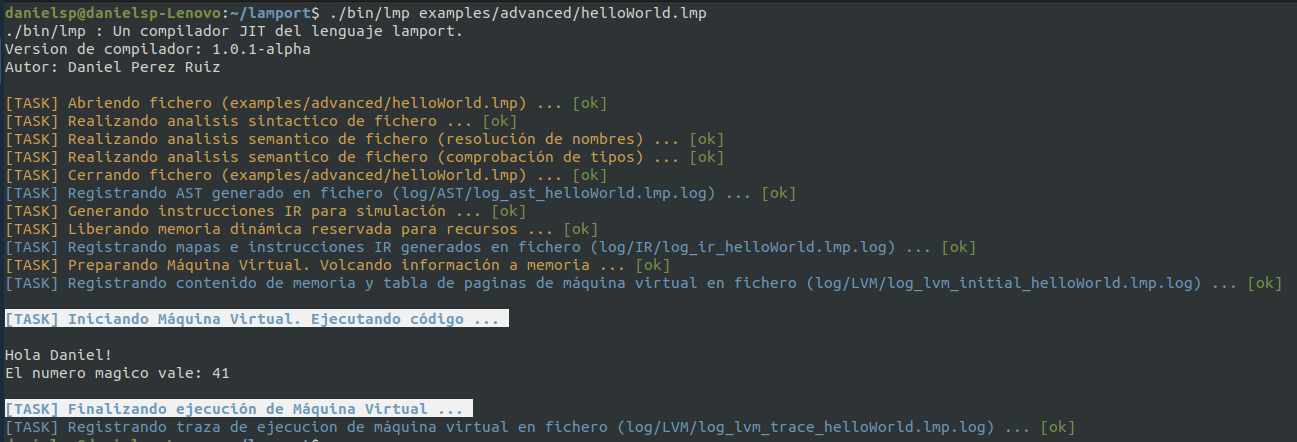
\includegraphics[width=\linewidth]{images/implementacion/ejecucion/lmp_hola_mundo.png}
    \caption{Ejecución de ``HolaMundo'' en el intérprete.}
    \label{fig:ejecucionHolaMundo}
\end{figure}

\begin{figure}[h]
    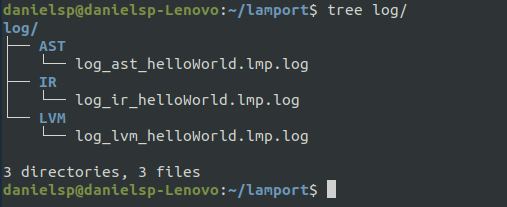
\includegraphics[width=\linewidth]{images/implementacion/ejecucion/logs.png}
    \caption{Ficheros de logging generados tras la ejecución.}
    \label{fig:logsHolaMundo}
\end{figure}

\section{Dockerización del intérprete}
Con la evolución constante de la tecnología y las infraestructuras de software, la necesidad de crear aplicaciones portables y escalables ha cobrado mayor importancia. Docker, una herramienta que permite la creación de contenedores, surge como una solución a esta demanda. Un contenedor Docker encapsula una aplicación junto con todas sus dependencias en una unidad estándar de software, garantizando que la aplicación se ejecute de la misma manera sin importar dónde se despliegue. 

\vspace{0.5cm}

En el contexto del intérprete desarrollado, la dockerización ofrece ventajas significativas en términos de portabilidad, aislamiento y replicabilidad. Esta sección detallará el proceso y las consideraciones adoptadas al dockerizar el intérprete, permitiendo su distribución y ejecución de manera homogénea en diferentes entornos.

\subsection{Construcción del contenedor}
Para construir el contenedor Docker que encapsulará el intérprete junto con todas sus dependencias, se han realizado las siguientes tareas:

\begin{enumerate}
    \item Elección de una imagen base. Ésta debe ser del menor tamaño posible para que sólo contenga lo imprescindible, además de ser una imagen que reciba constantes actualizaciones de seguridad y mantenimiento. En el caso de este proyecto, \textbf{alpine} es una excelente elección por cumplir estas dos características.
    \item Construir el fichero \code{Dockerfile}. Este fichero indica cómo se debe construir el contenedor de forma automática, aprovisionándolo de todas las dependencias.
    \item Definir script de ejecución utilizando el contenedor virtual. Para hacer aún más fácil el uso de esta herramienta se definió un script denominado \code{./lmp_docker.sh} que ejecuta el contenedor utilizando como argumento el fichero de código Lamport indicado.
\end{enumerate}

\subsection{Compilación estática del intérprete}
La compilación estática se refiere al proceso de integrar todas las bibliotecas y dependencias requeridas por una aplicación directamente en el binario ejecutable, en lugar de depender de bibliotecas compartidas en el sistema en tiempo de ejecución. Este método tiene varias ventajas, especialmente en el contexto que concierne a esta sección:

\begin{itemize}
\item \textbf{Portabilidad mejorada}: Un binario estáticamente enlazado no tiene dependencias externas, lo que garantiza que funcionará en cualquier entorno que lo ejecute, eliminando así problemas relacionados con versiones de bibliotecas o dependencias faltantes.
\item \textbf{Reducción del tamaño del contenedor}: Al no requerir la instalación de bibliotecas adicionales en el contenedor (sólo se necesita instalar flex y bison de manera inevitable), el tamaño de la imagen resultante puede reducirse significativamente. En este proyecto, la imagen del contenedor se redujo de 249 MB a tan solo 24 MB, una optimización impresionante.
\item \textbf{Seguridad mejorada}: Al reducir el número de componentes en el contenedor, se disminuye la superficie de ataque potencial, al eliminar software adicional que no es esencial para la aplicación pero que podría presentar vulnerabilidades.
\end{itemize}

Para lograr la compilación estática del intérprete, se utilizaron las herramientas gcc y g++ con las opciones de enlazado estático. Además, se aprovechó el enfoque de construcción multi-etapa en Docker, donde la primera etapa incluye todas las herramientas y dependencias necesarias para la compilación, y la segunda etapa simplemente copia el binario resultante, resultando en una imagen Docker final limpia y optimizada.

\begin{figure}[h]
    \begin{adjustbox}{center}
        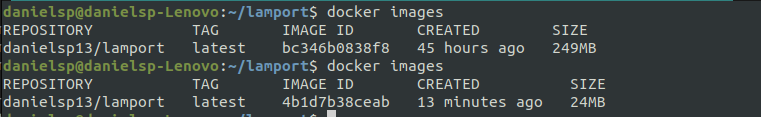
\includegraphics[width=7.0in]{images/implementacion/docker/docker_reduce.png}
    \end{adjustbox}
    \caption{Tamaño de contenedor docker antes y después de usar compilación estática.}
    \label{fig:DockerReduce}
\end{figure}